
%%%----------------------------------------------------------
%%%----------------------------------------------------------
%%%----------------------------------------------------------
%%%----------------------------------------------------------
%%%----------------------------------------------------------
\chapter{Walking}
%%%----------------------------------------------------------

The activity "walking" will be analyzed here with graphics.
%%%----------------------------------------------------------
\section{Test case 1}
%%%----------------------------------------------------------
Test case 1 in Fig.~\ref{fig:Test_case_1_walking}
\begin{figure}
	\centering\small
	\setlength{\tabcolsep}{0mm}	% alle Spaltenränder auf 0mm
	\begin{tabular}{c@{\hspace{12mm}}c} % mittlerer Abstand = 12mm
		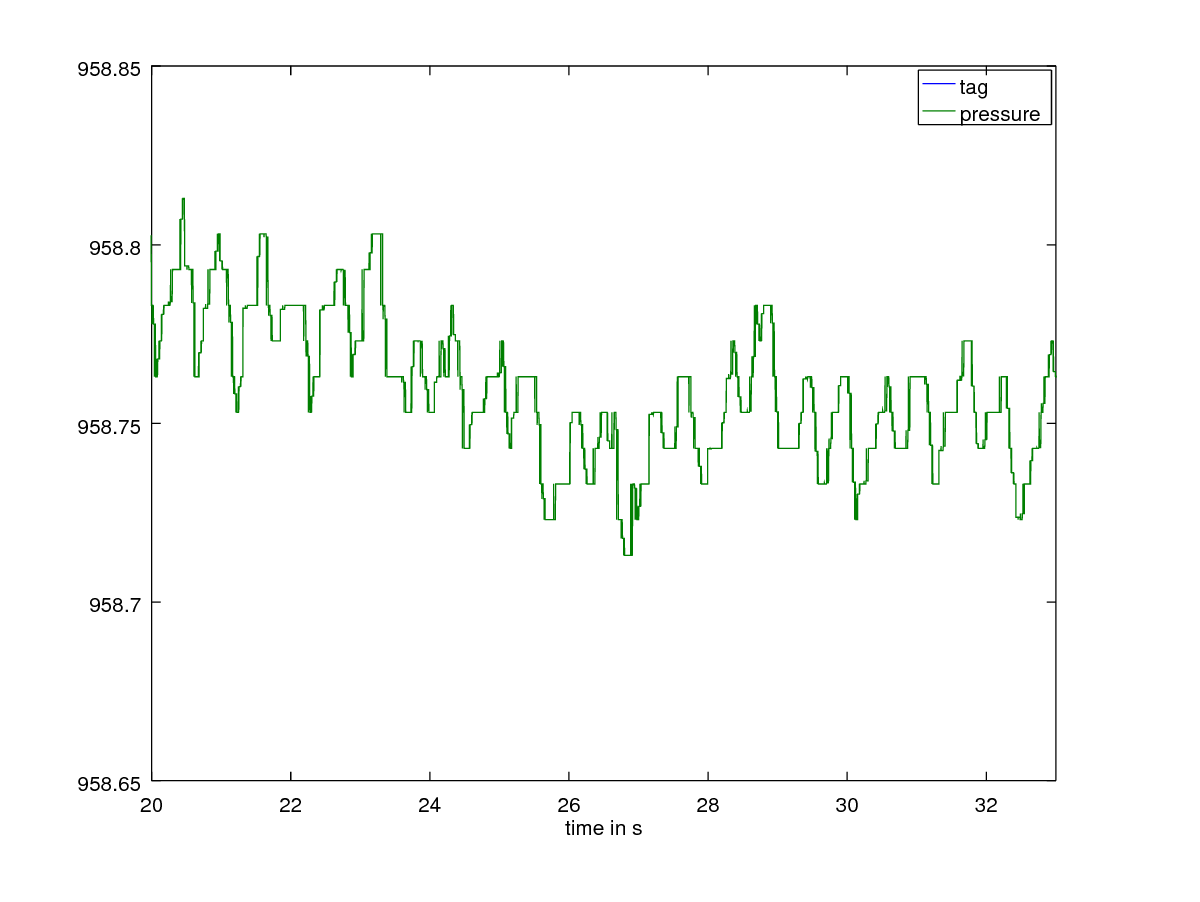
\includegraphics[width=.45\textwidth]{stairsfhdown_walking_p} &
		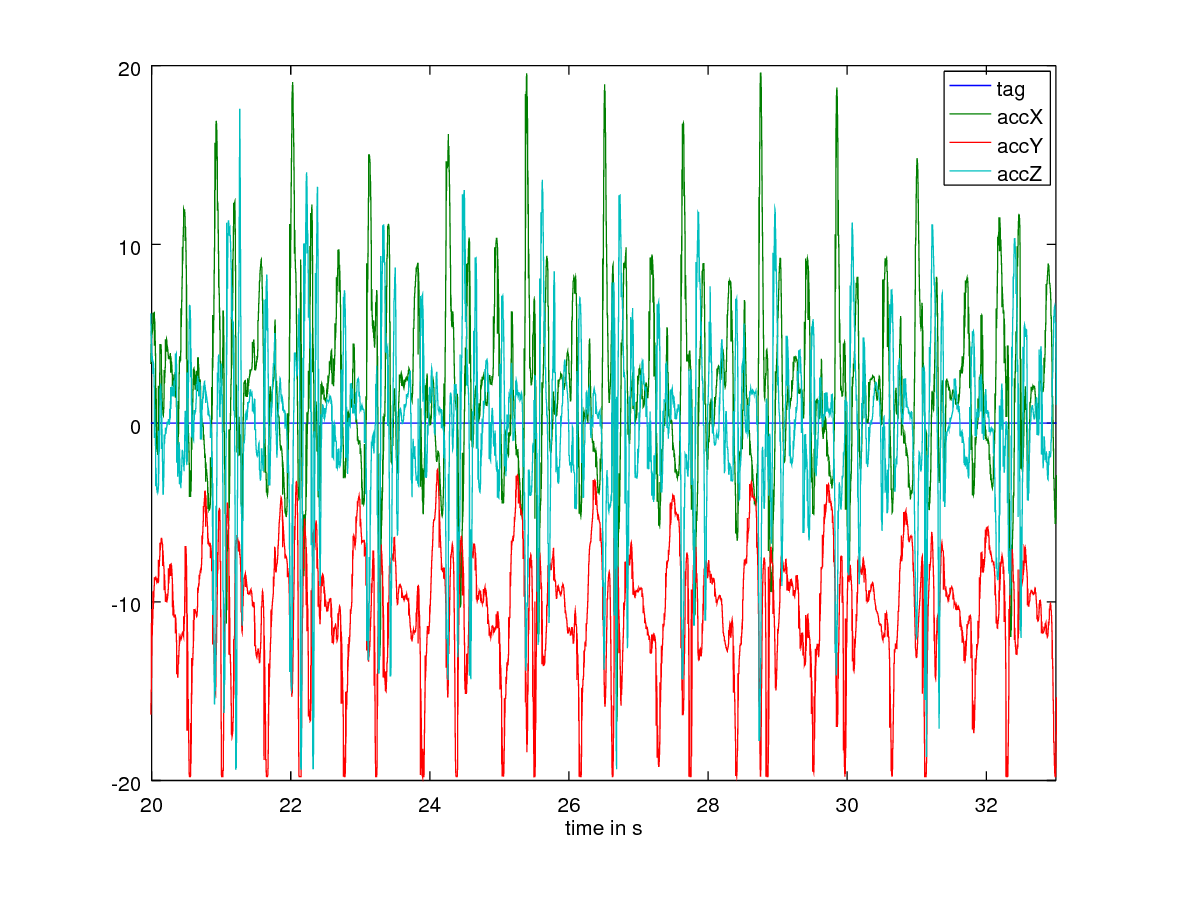
\includegraphics[width=.45\textwidth]{stairsfhdown_walking_a} 
		\\
		(a) & (b)
		\\[4pt]	%vertical extra spacing (4 points)
		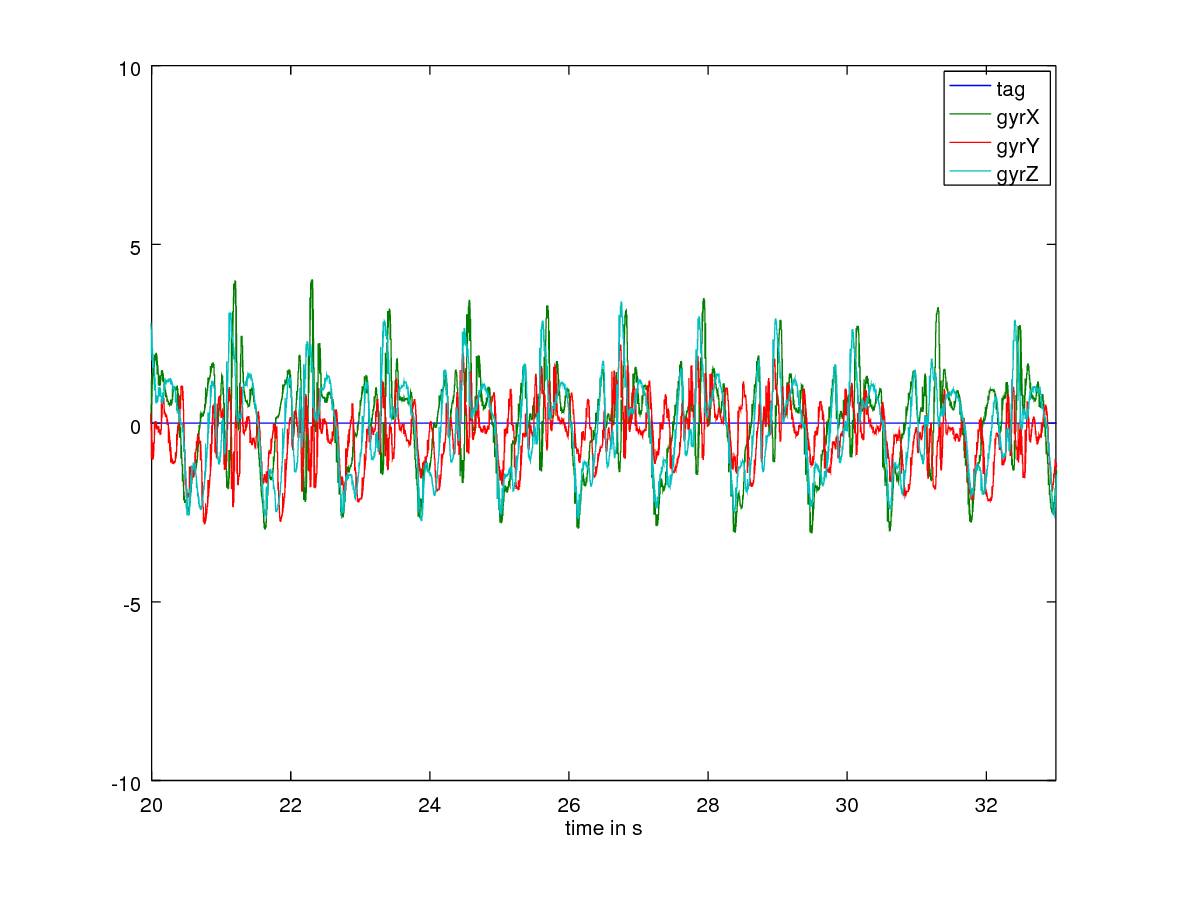
\includegraphics[width=.45\textwidth]{stairsfhdown_walking_g} &
		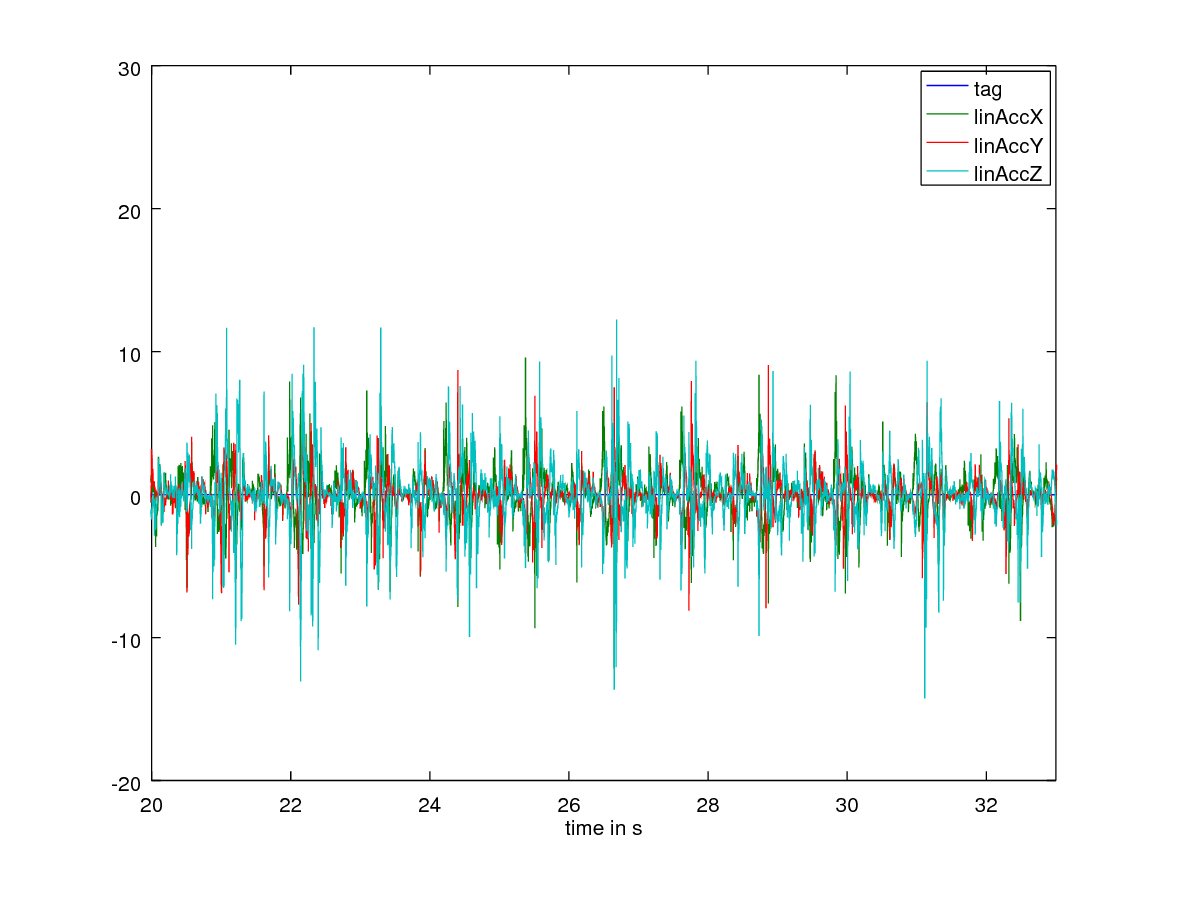
\includegraphics[width=.45\textwidth]{stairsfhdown_walking_la} 
		\\
		(c) & (d)
		\\[4pt]	%vertical extra spacing (4 points)
		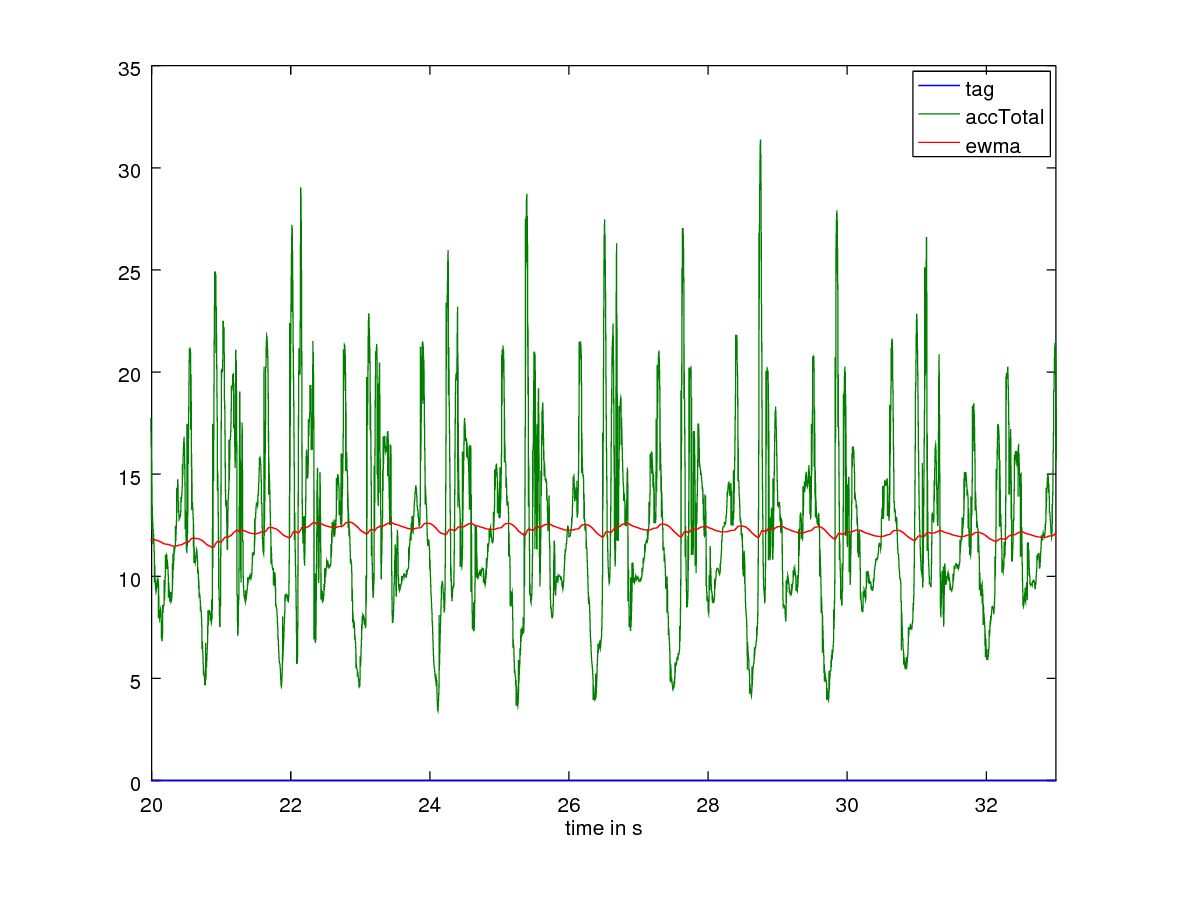
\includegraphics[width=.45\textwidth]{stairsfhdown_walking_atotal} &
		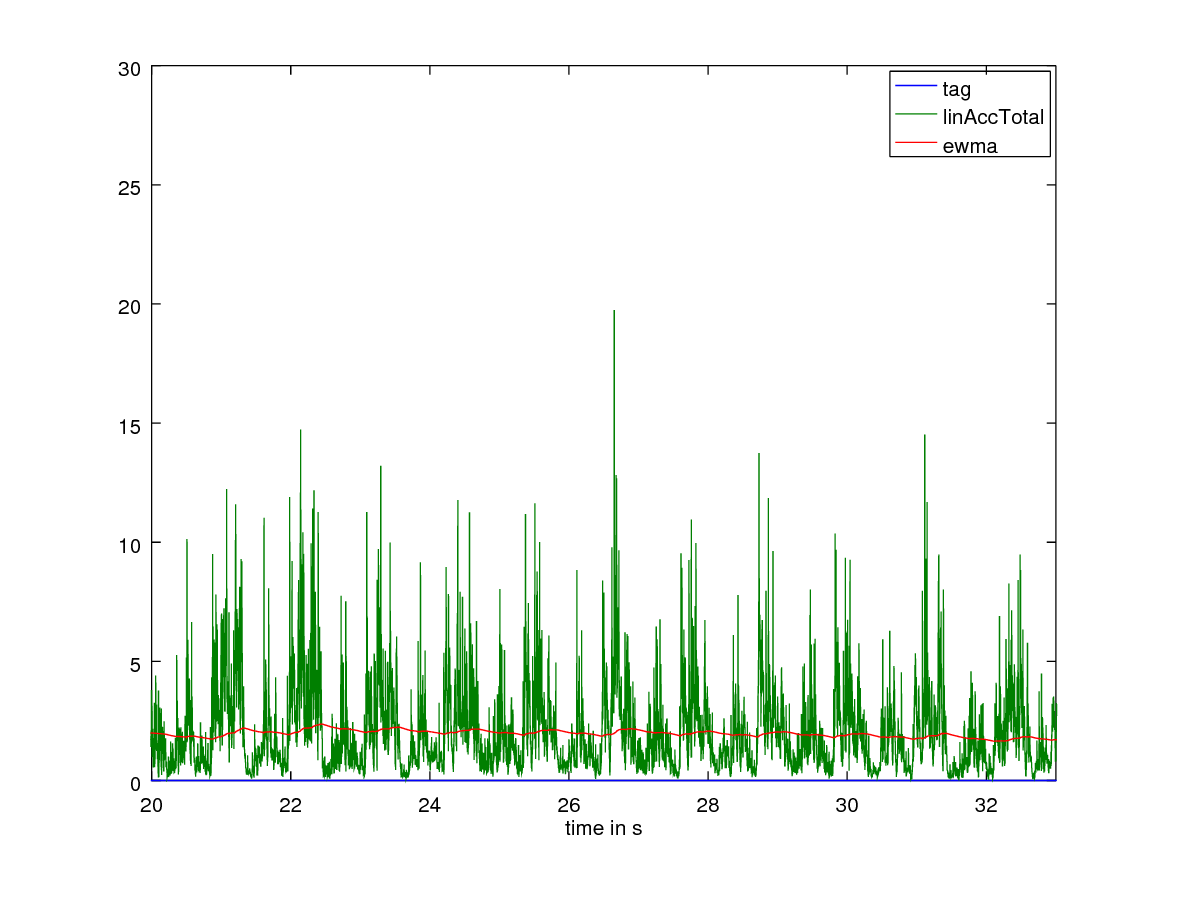
\includegraphics[width=.45\textwidth]{stairsfhdown_walking_latotal} 
		\\
		(e) & (f)
	\end{tabular}
	%
	\caption{Test case 1}
	\label{fig:Test_case_1_walking}
\end{figure}

%%%----------------------------------------------------------
\section{Test case 2}
%%%----------------------------------------------------------

Test case 2 in Fig.~\ref{fig:Test_case_2_walking}
\begin{figure}
	\centering\small
	\setlength{\tabcolsep}{0mm}	% alle Spaltenränder auf 0mm
	\begin{tabular}{c@{\hspace{12mm}}c} % mittlerer Abstand = 12mm
	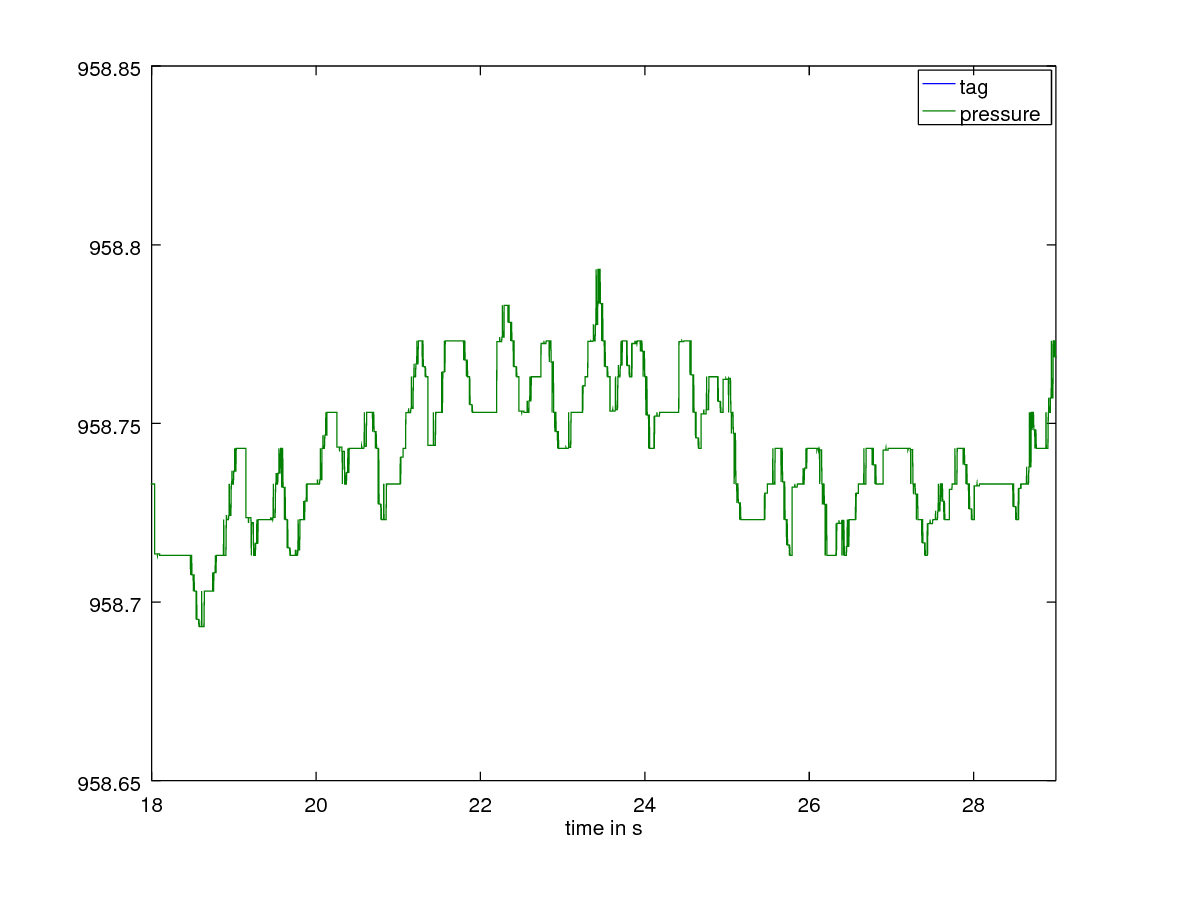
\includegraphics[width=.45\textwidth]{stairsfhdown2_walking_p} &
	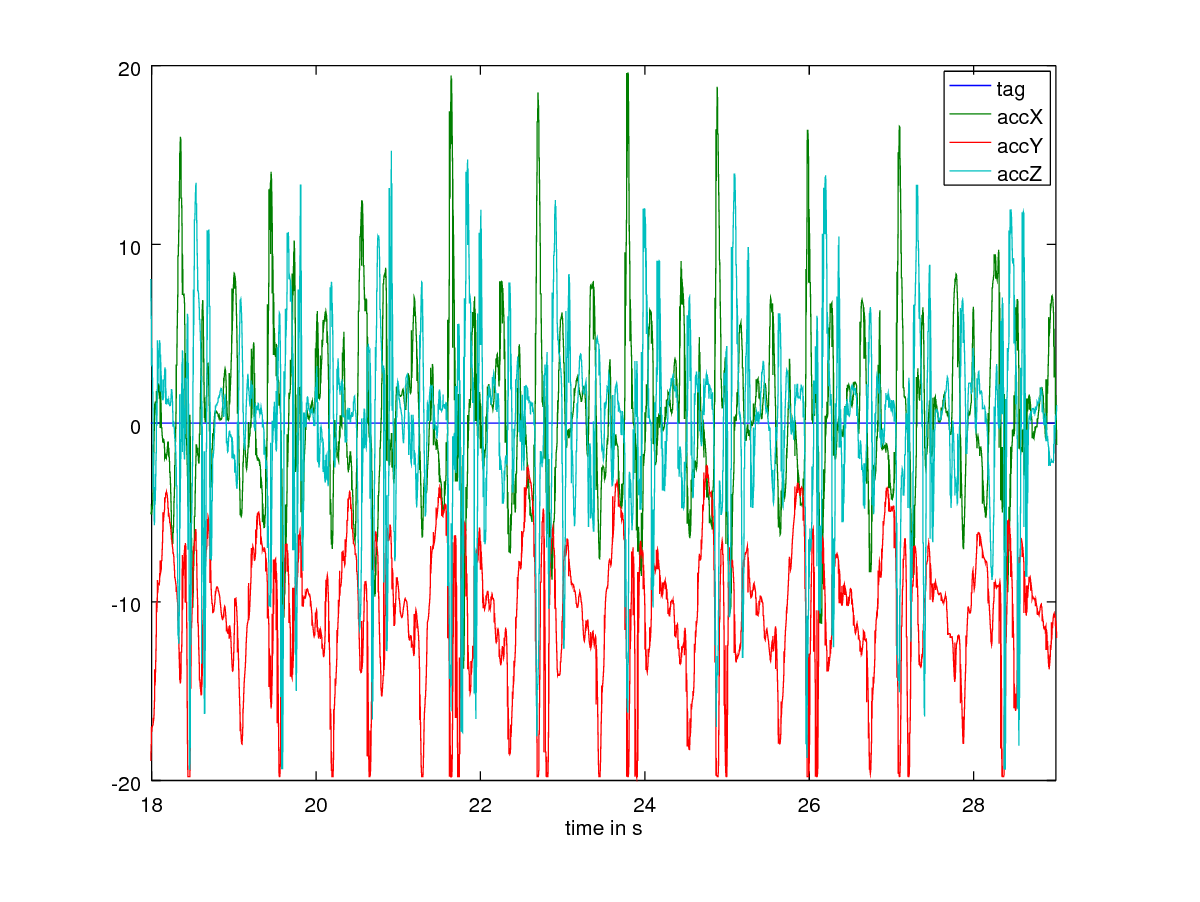
\includegraphics[width=.45\textwidth]{stairsfhdown2_walking_a} 
	\\
	(a) & (b)
	\\[4pt]	%vertical extra spacing (4 points)
	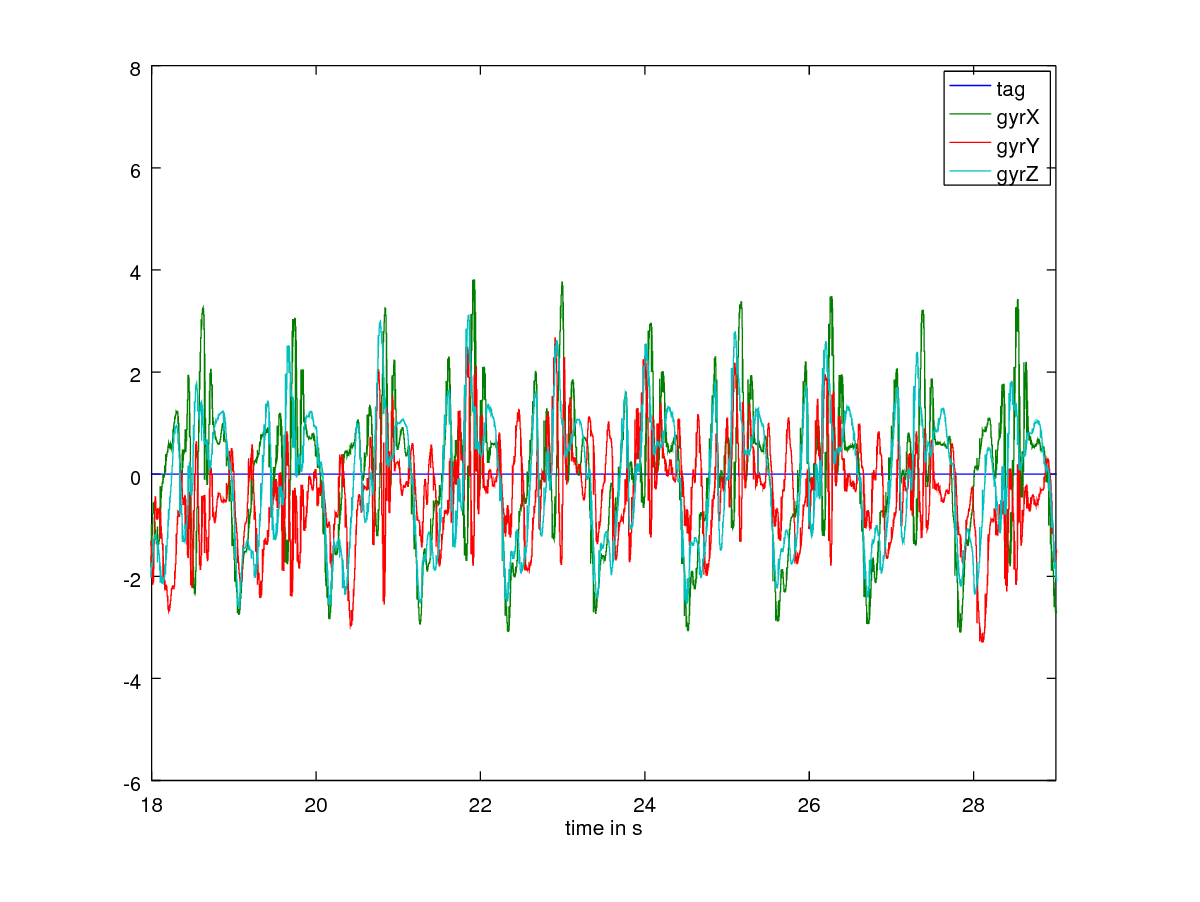
\includegraphics[width=.45\textwidth]{stairsfhdown2_walking_g} &
	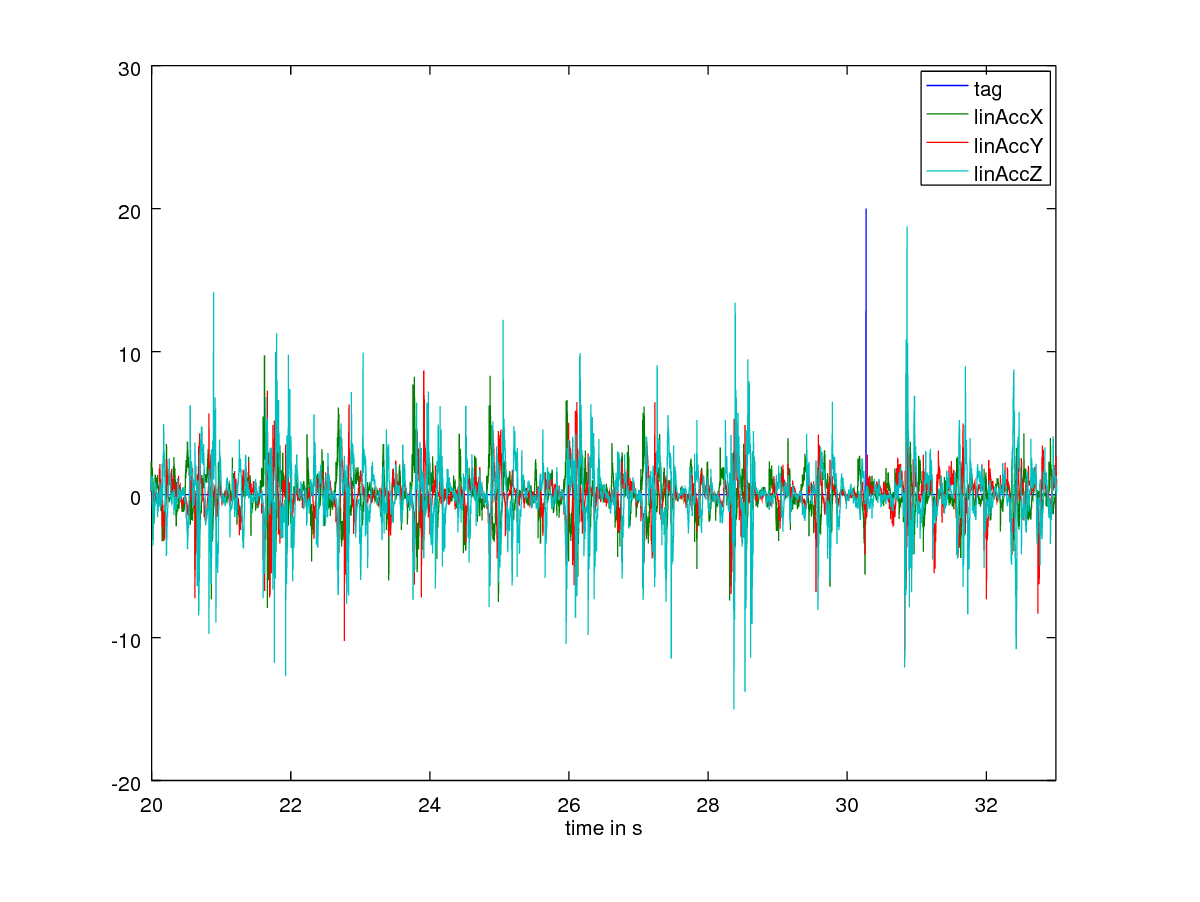
\includegraphics[width=.45\textwidth]{stairsfhdown2_walking_la} 
	\\
	(c) & (d)
	\\[4pt]	%vertical extra spacing (4 points)
	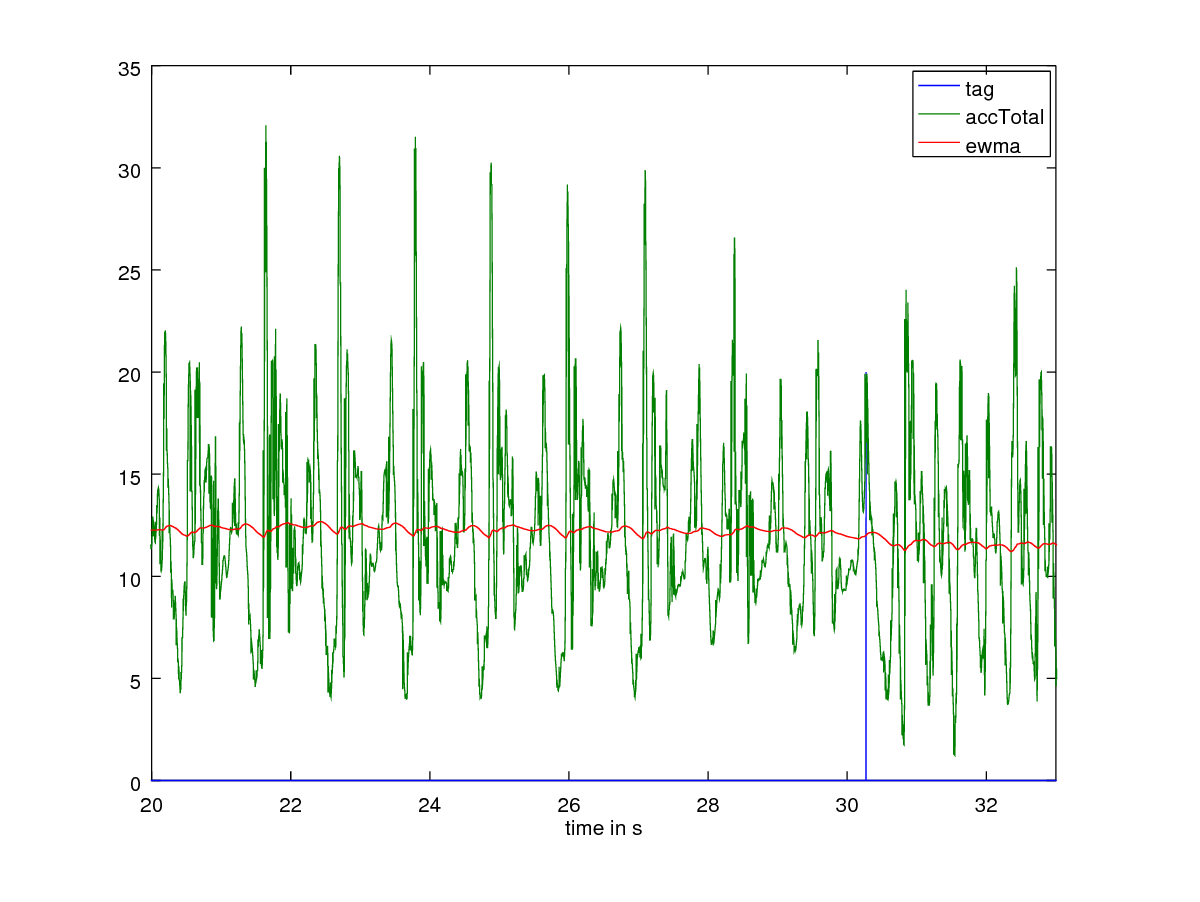
\includegraphics[width=.45\textwidth]{stairsfhdown2_walking_atotal} &
	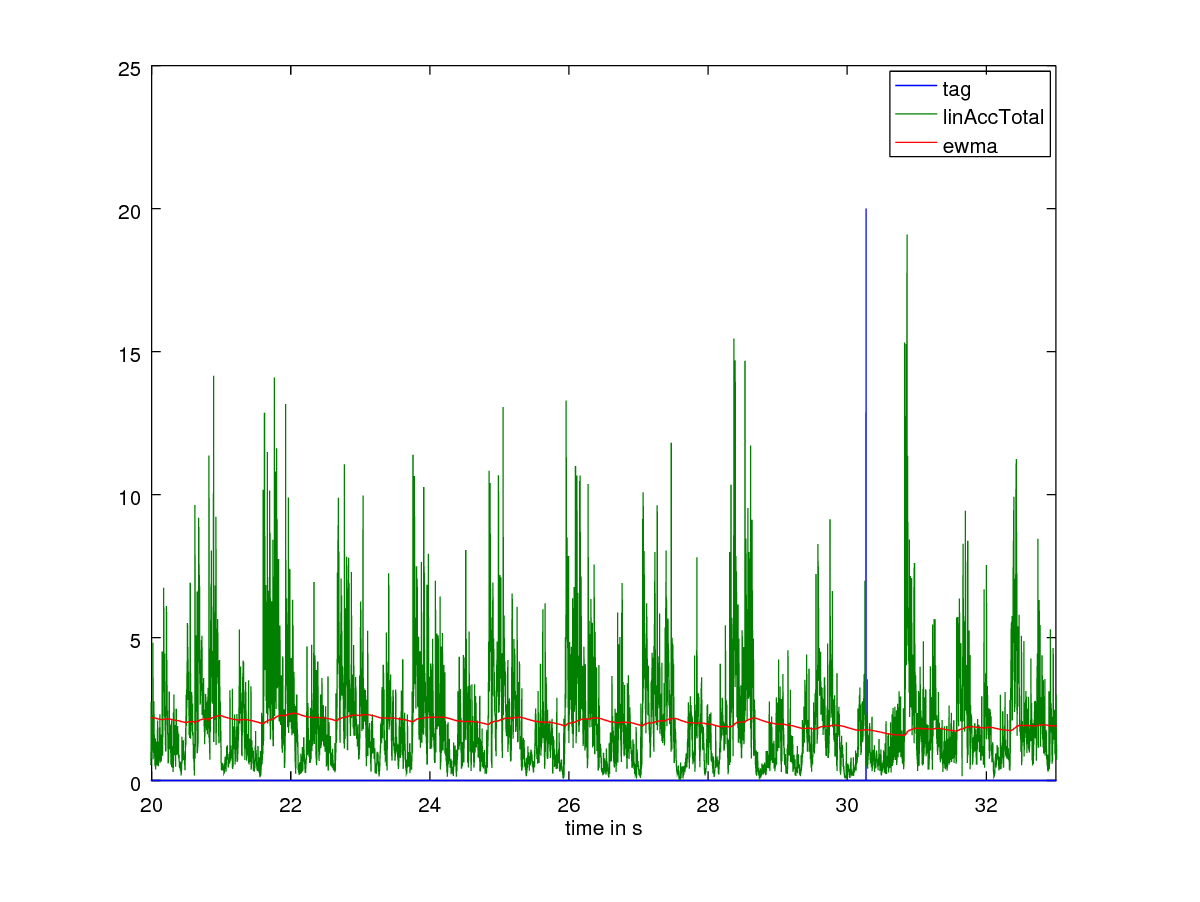
\includegraphics[width=.45\textwidth]{stairsfhdown2_walking_latotal} 
	\\
	(e) & (f)
	\end{tabular}
	%
	\caption{Test case 2}
	\label{fig:Test_case_2_walking}
\end{figure}


%%%----------------------------------------------------------
\section{Test case 3}
%%%----------------------------------------------------------
Test case 3 in Fig.~\ref{fig:Test_case_3_walking}
\begin{figure}
	\centering\small
	\setlength{\tabcolsep}{0mm}	% alle Spaltenränder auf 0mm
	\begin{tabular}{c@{\hspace{12mm}}c} % mittlerer Abstand = 12mm
	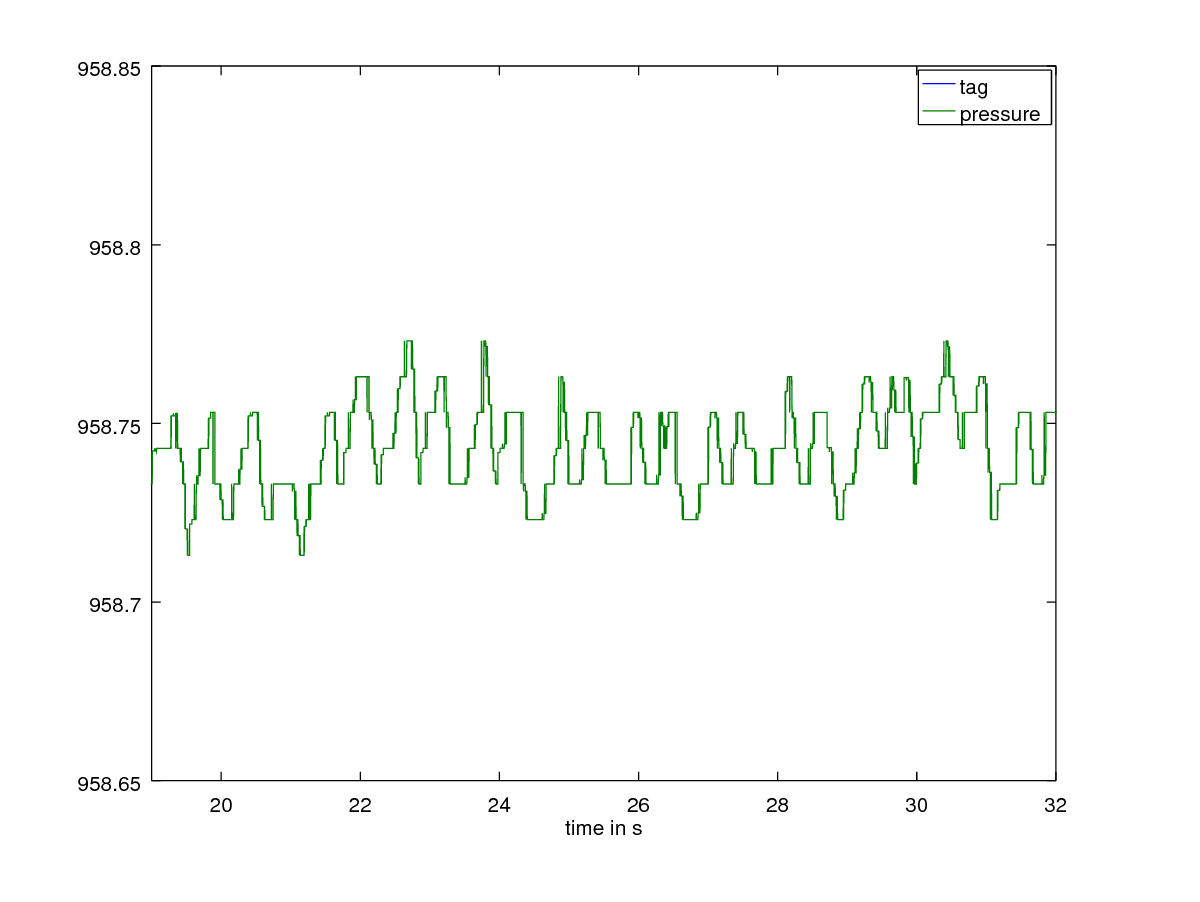
\includegraphics[width=.45\textwidth]{stairsfhdown6_walking_p} &
	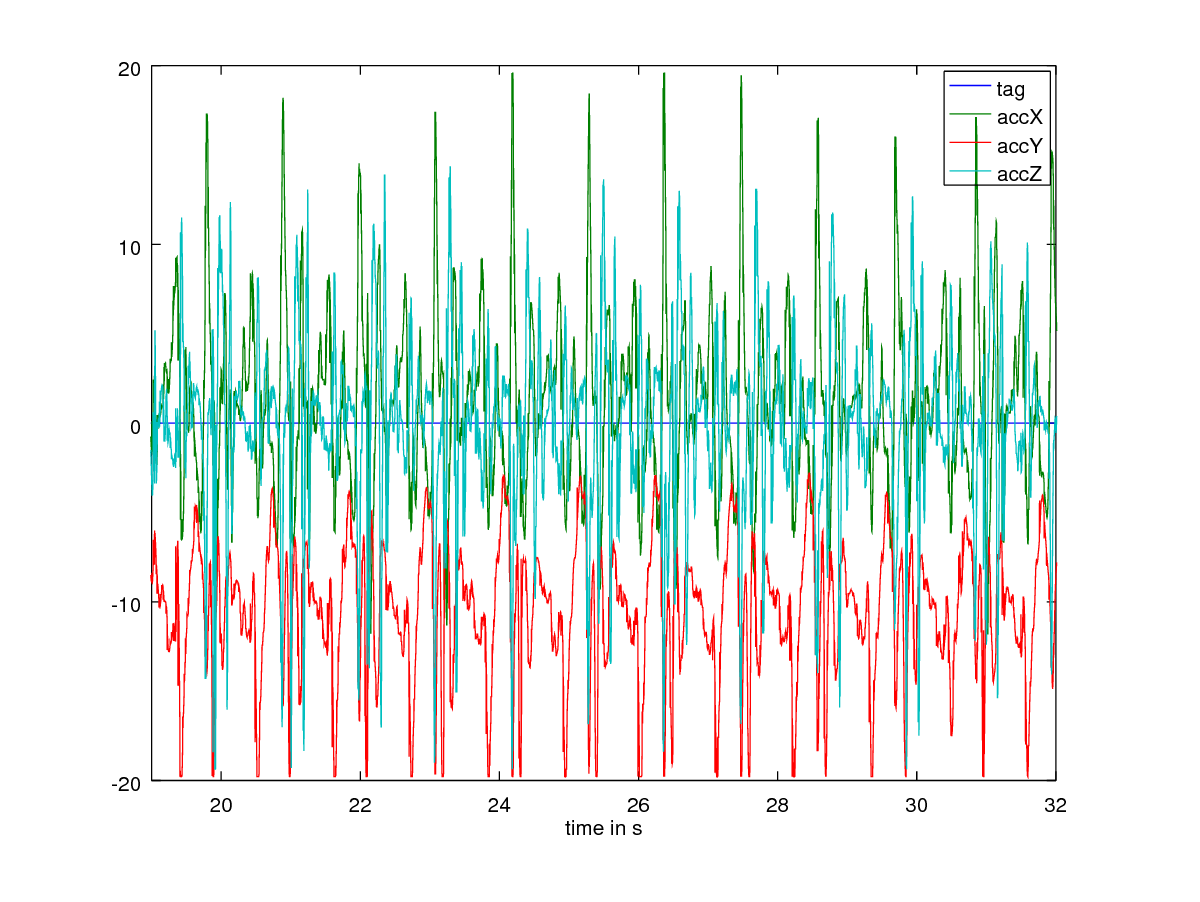
\includegraphics[width=.45\textwidth]{stairsfhdown6_walking_a} 
	\\
	(a) & (b)
	\\[4pt]	%vertical extra spacing (4 points)
	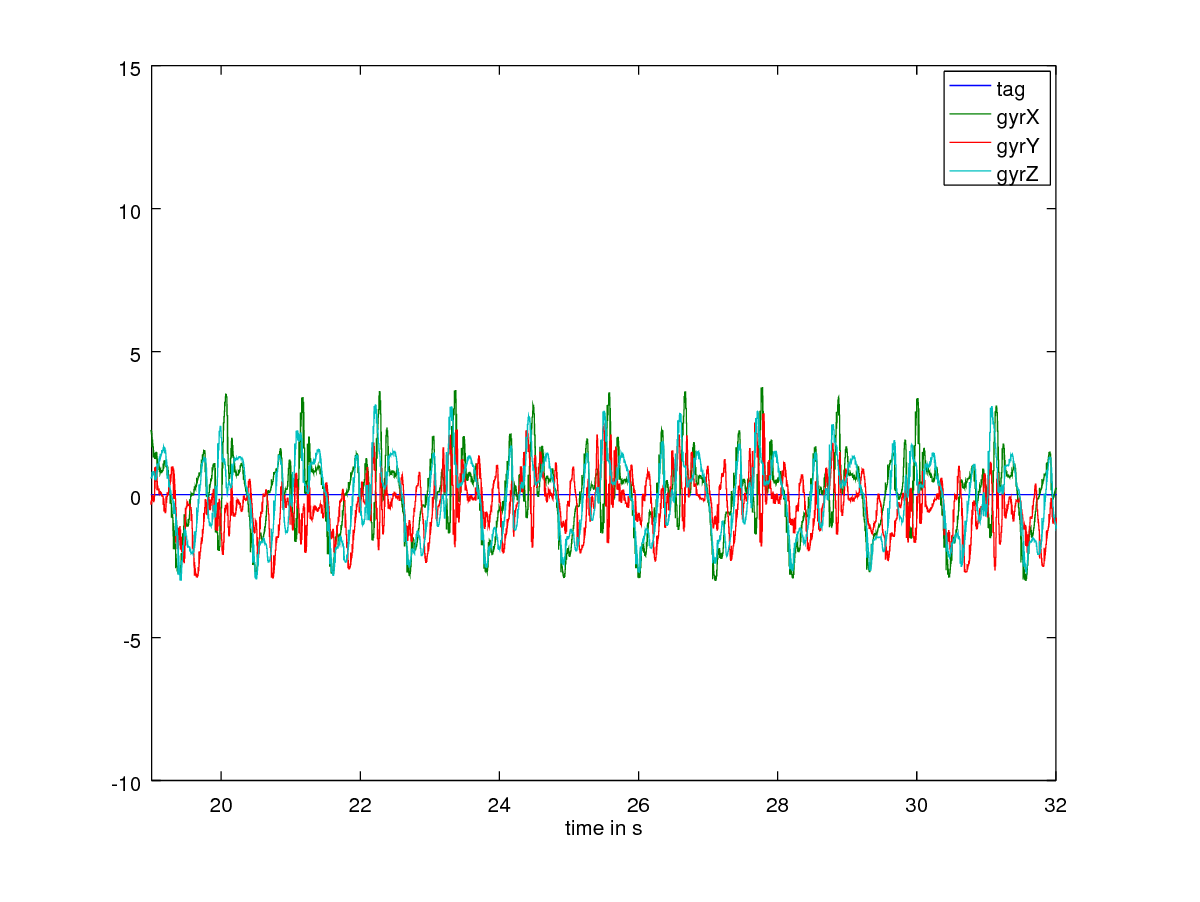
\includegraphics[width=.45\textwidth]{stairsfhdown6_walking_g} &
	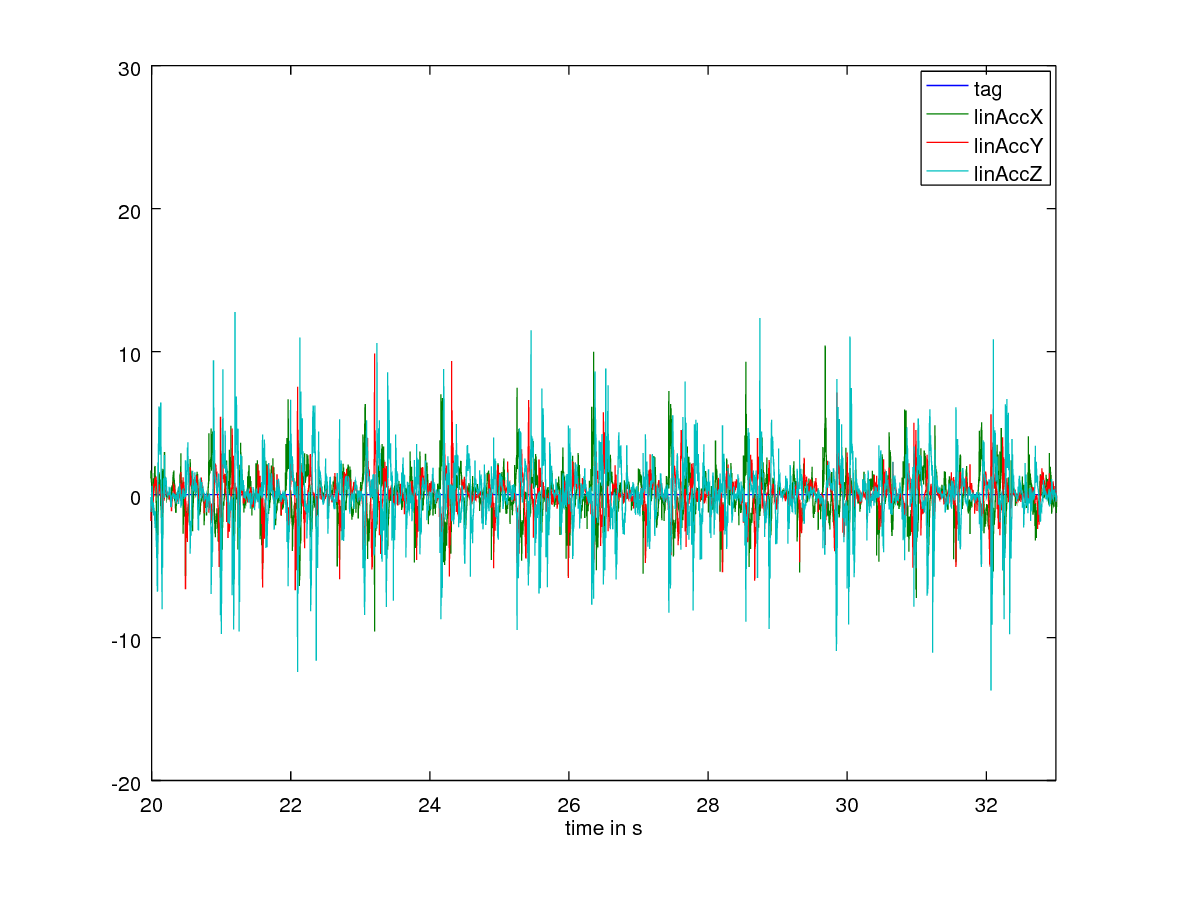
\includegraphics[width=.45\textwidth]{stairsfhdown6_walking_la} 
	\\
	(c) & (d)
	\\[4pt]	%vertical extra spacing (4 points)
	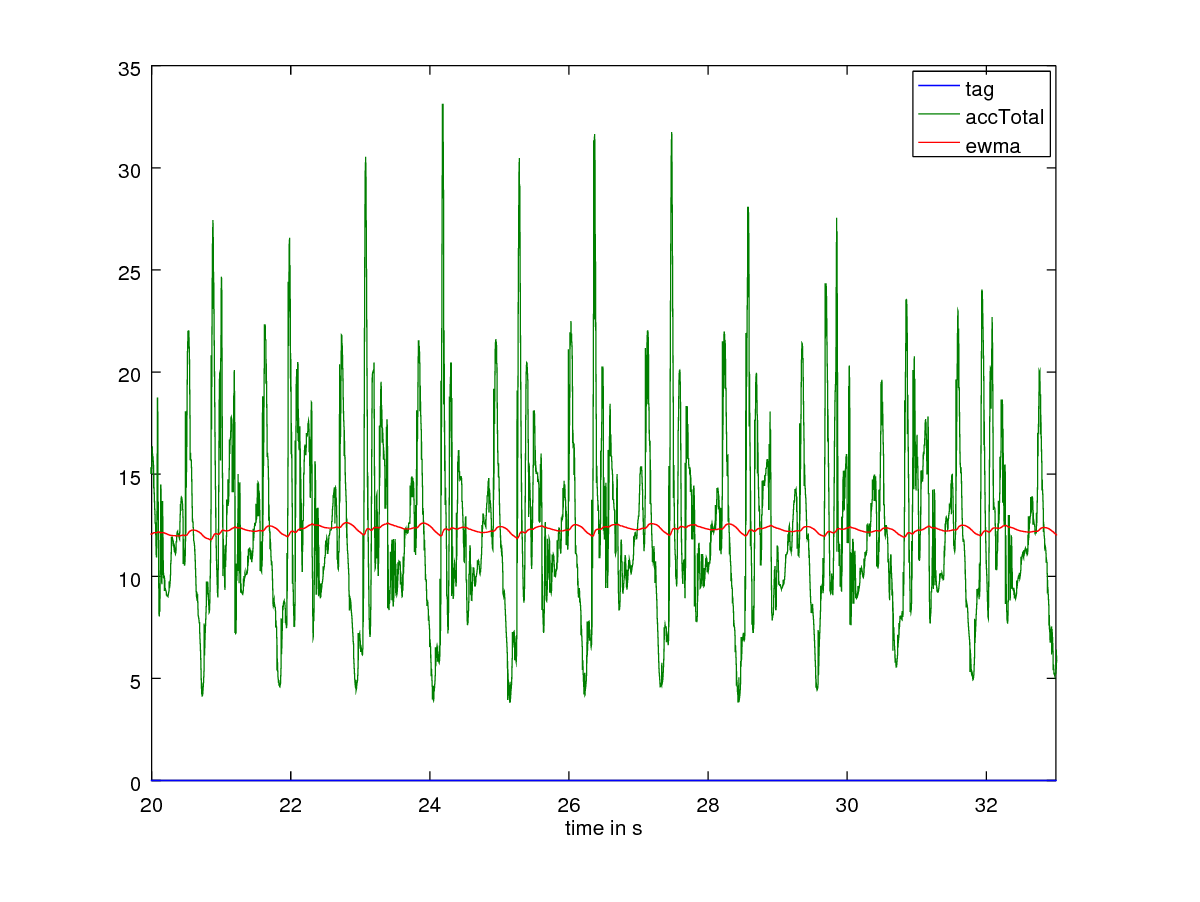
\includegraphics[width=.45\textwidth]{stairsfhdown6_walking_atotal} &
	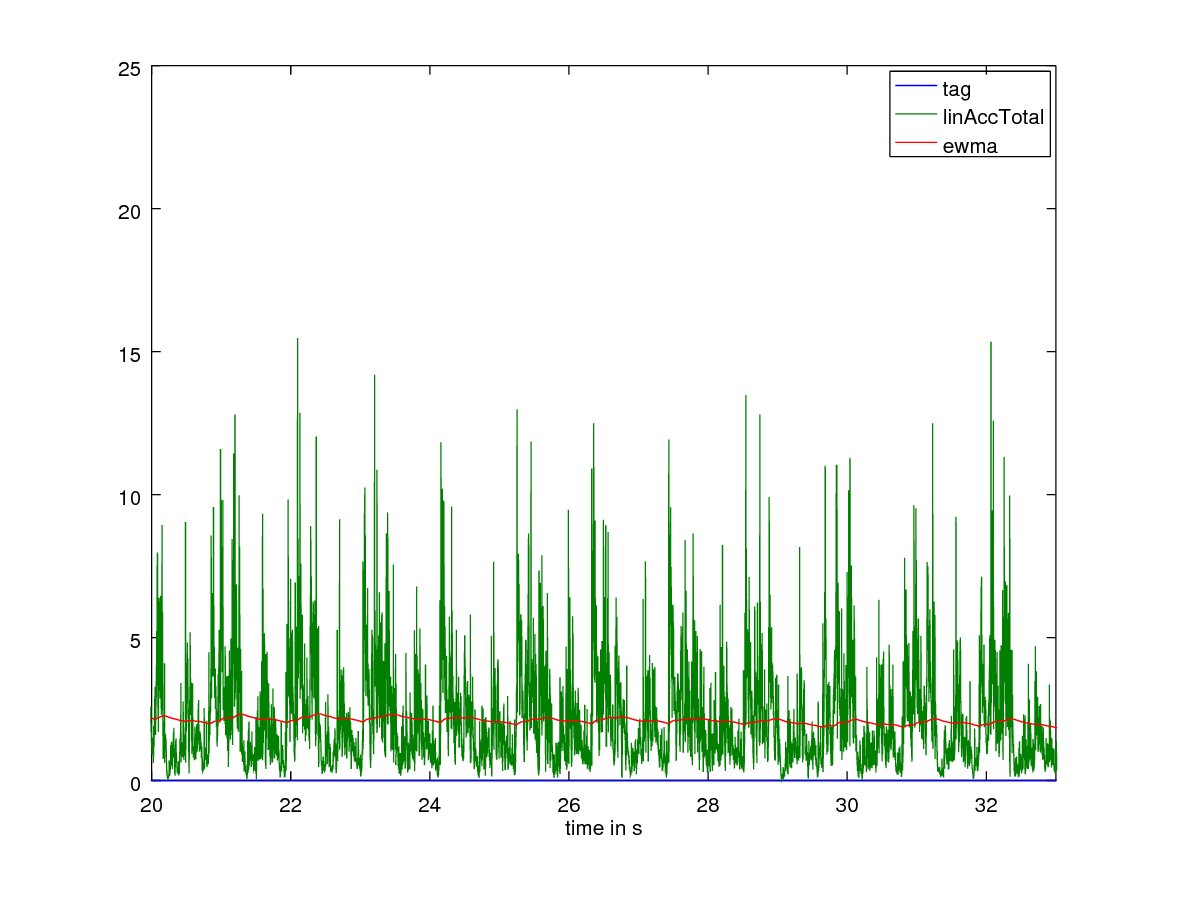
\includegraphics[width=.45\textwidth]{stairsfhdown6_walking_latotal} 
	\\
	(e) & (f)
	\end{tabular}
	%
	\caption{Test case 3}
	\label{fig:Test_case_3_walking}
\end{figure}

%%%----------------------------------------------------------
\section{Test case 4}
%%%----------------------------------------------------------
Test case 4 in Fig.~\ref{fig:Test_case_4_walking}
\begin{figure}
	\centering\small
	\setlength{\tabcolsep}{0mm}	% alle Spaltenränder auf 0mm
	\begin{tabular}{c@{\hspace{12mm}}c} % mittlerer Abstand = 12mm
	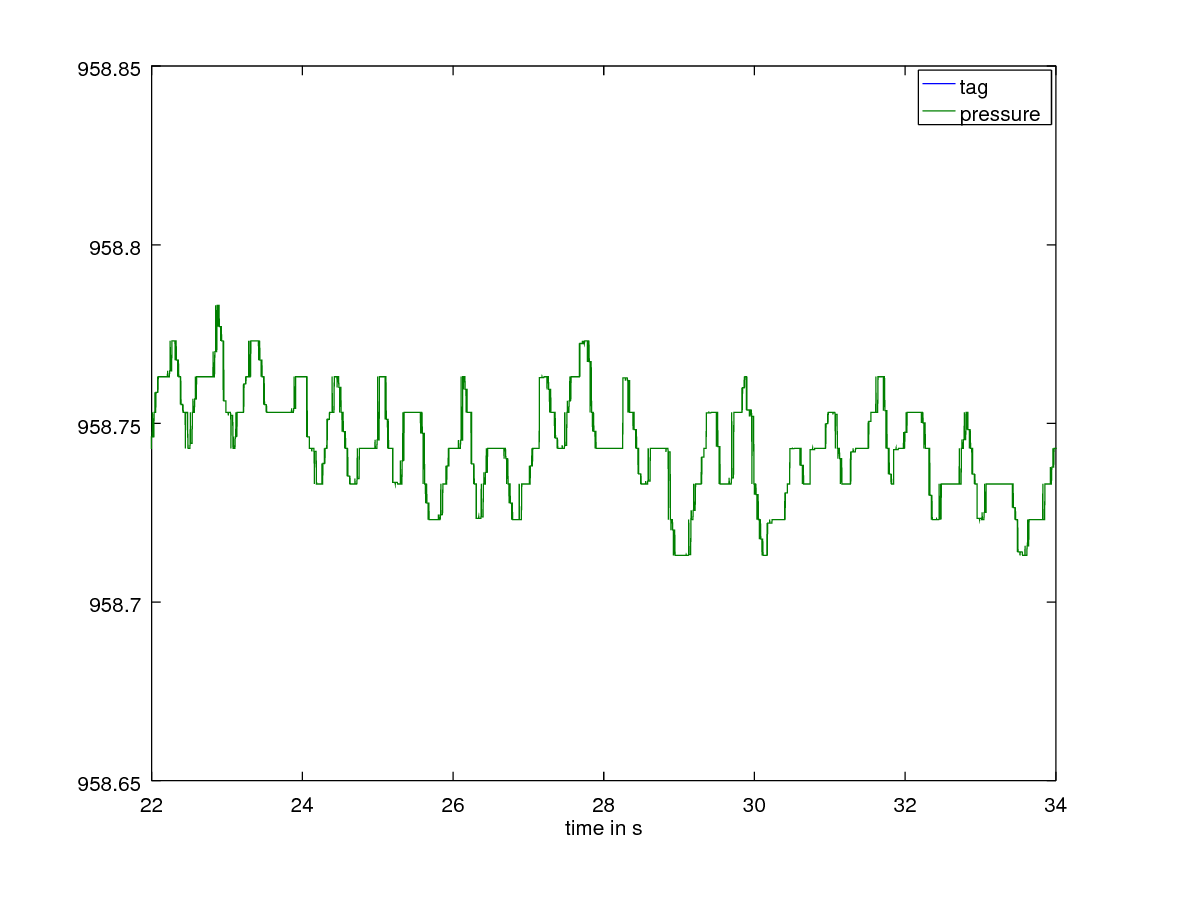
\includegraphics[width=.45\textwidth]{stairsfhdown10_walking_p} &
	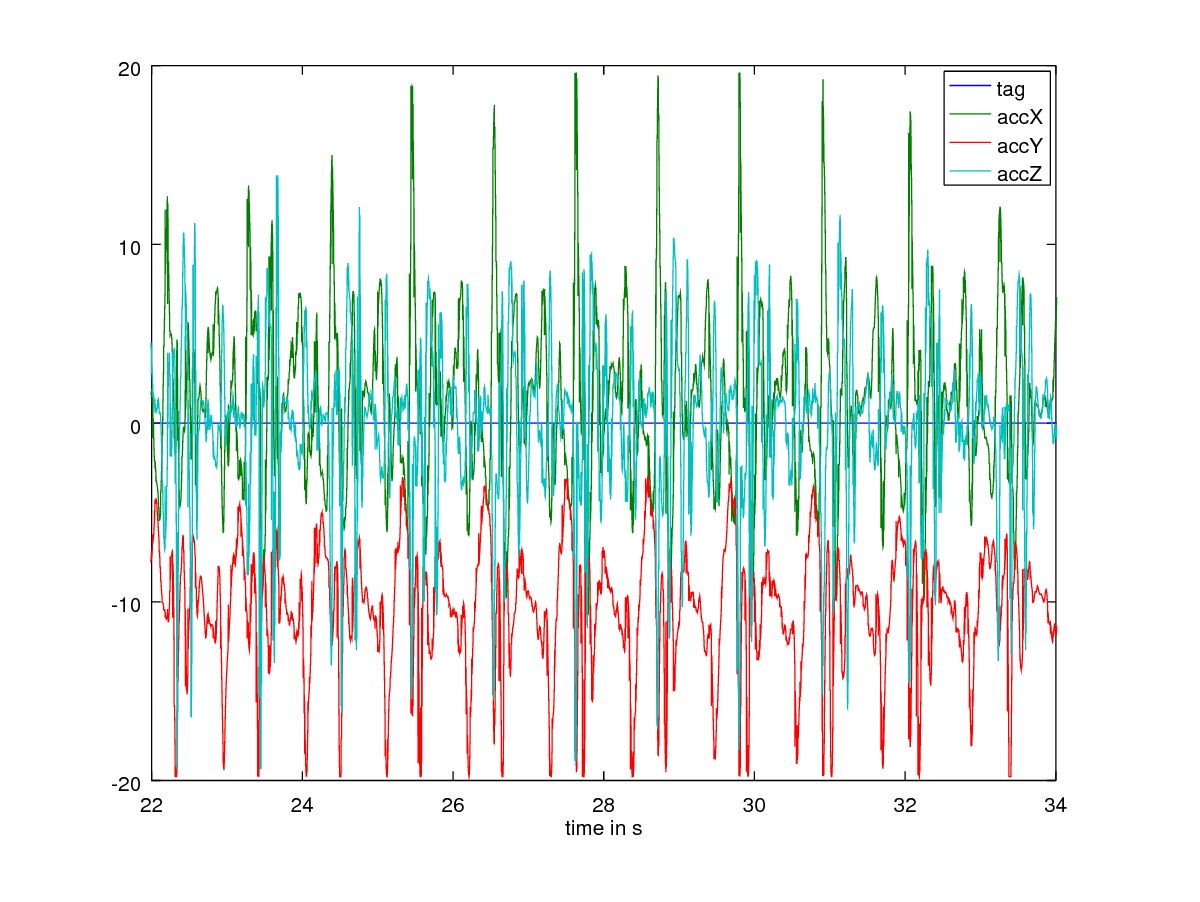
\includegraphics[width=.45\textwidth]{stairsfhdown10_walking_a} 
	\\
	(a) & (b)
	\\[4pt]	%vertical extra spacing (4 points)
	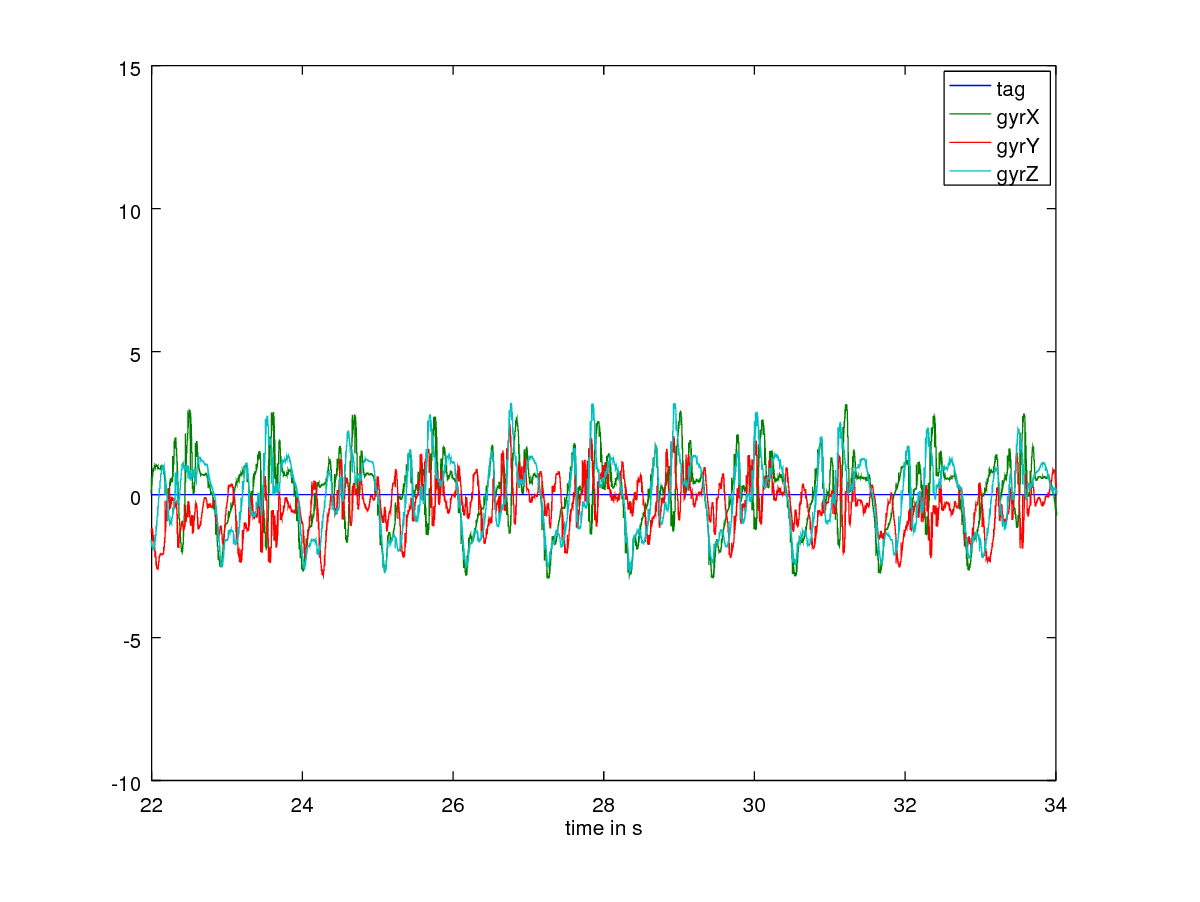
\includegraphics[width=.45\textwidth]{stairsfhdown10_walking_g} &
	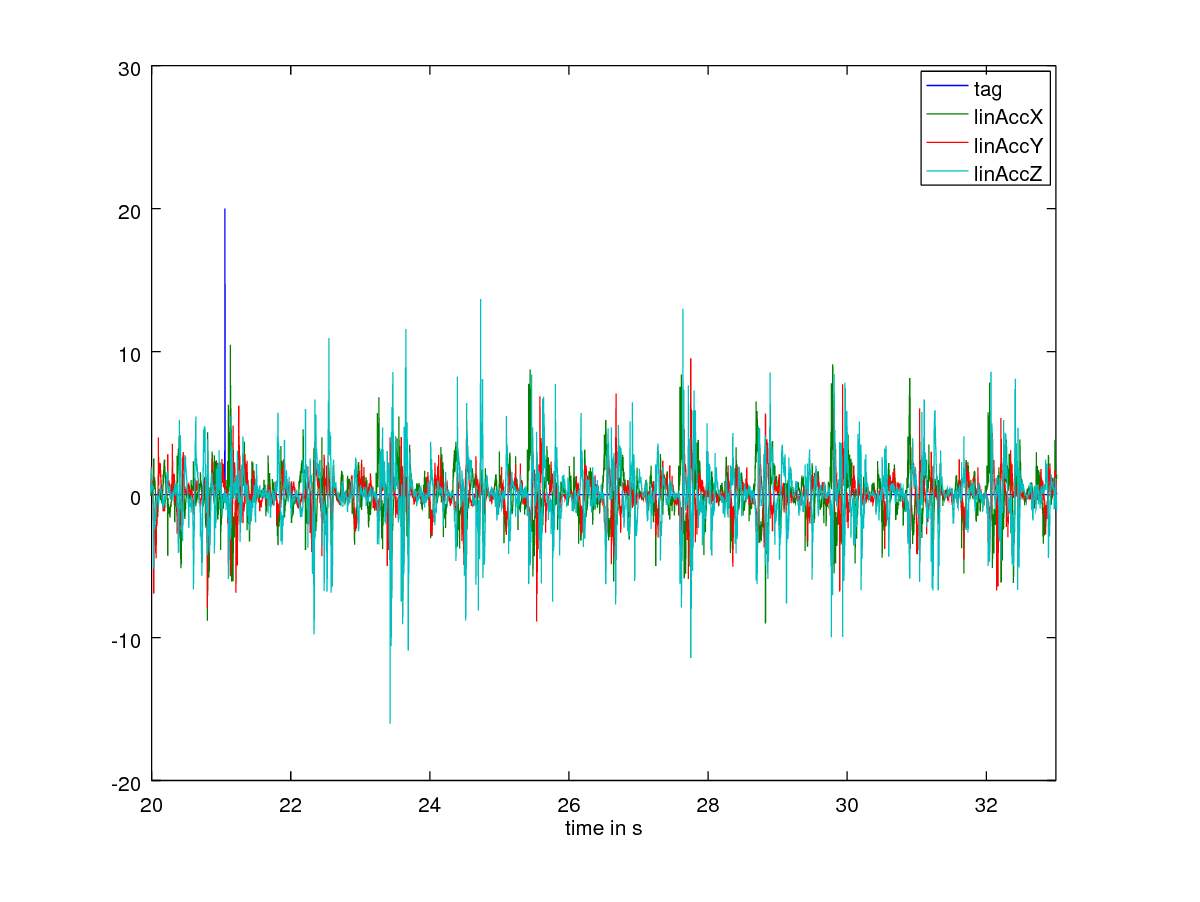
\includegraphics[width=.45\textwidth]{stairsfhdown10_walking_la} 
	\\
	(c) & (d)
	\\[4pt]	%vertical extra spacing (4 points)
	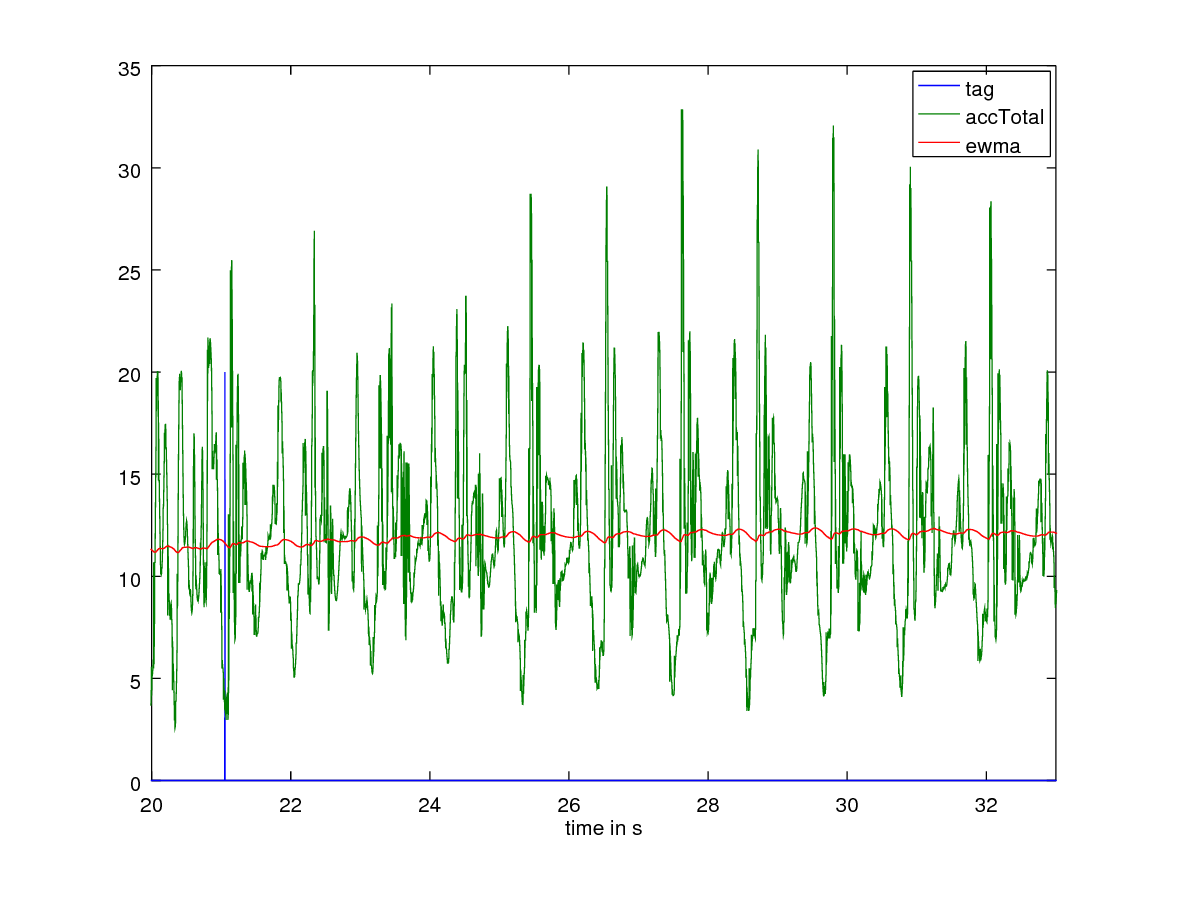
\includegraphics[width=.45\textwidth]{stairsfhdown10_walking_atotal} &
	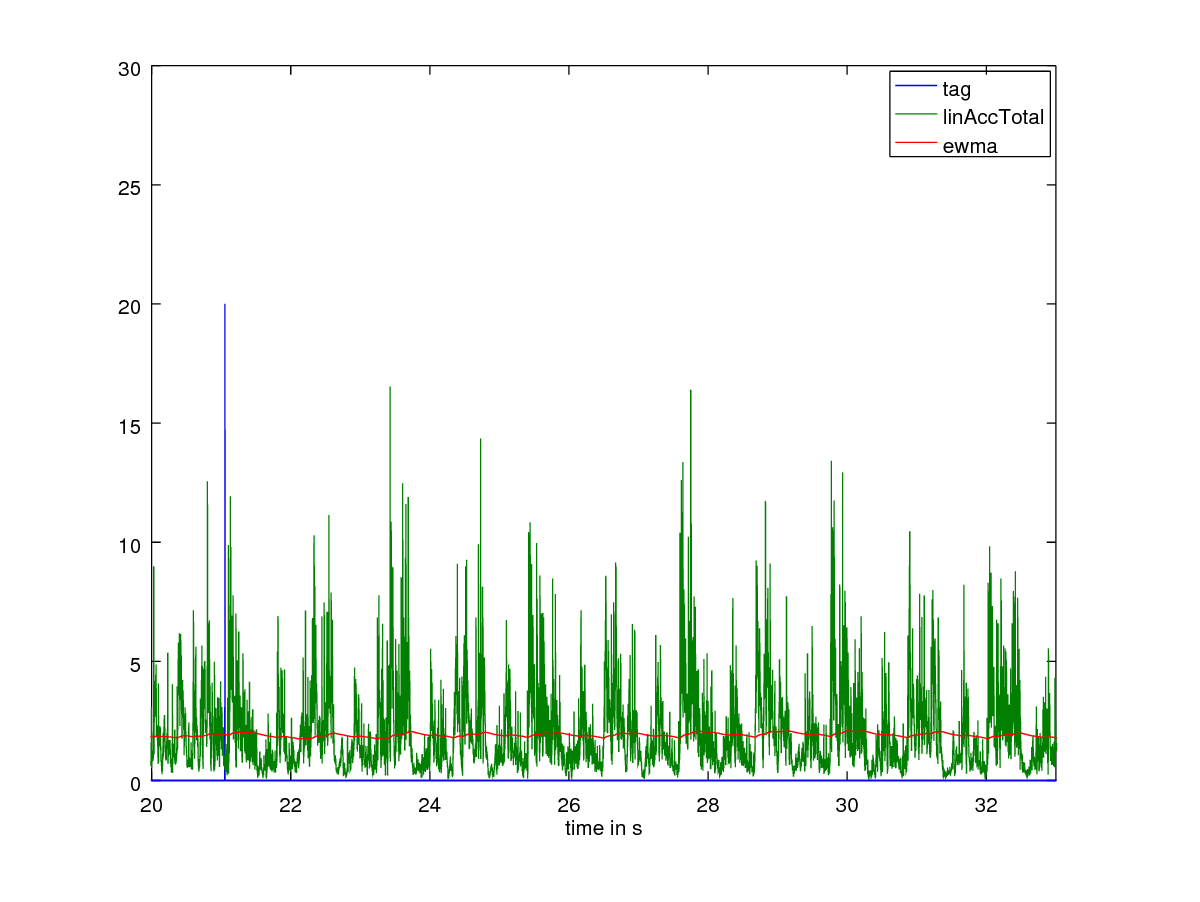
\includegraphics[width=.45\textwidth]{stairsfhdown10_walking_latotal} 
	\\
	(e) & (f)
		\end{tabular}
	%
	\caption{Test case 4}
	\label{fig:Test_case_4_walking}
\end{figure}

%%%----------------------------------------------------------
\section{Test case 5}
%%%----------------------------------------------------------
Test case 5 in Fig.~\ref{fig:Test_case_5_walking}
\begin{figure}
	\centering\small
	\setlength{\tabcolsep}{0mm}	% alle Spaltenränder auf 0mm
	\begin{tabular}{c@{\hspace{12mm}}c} % mittlerer Abstand = 12mm
		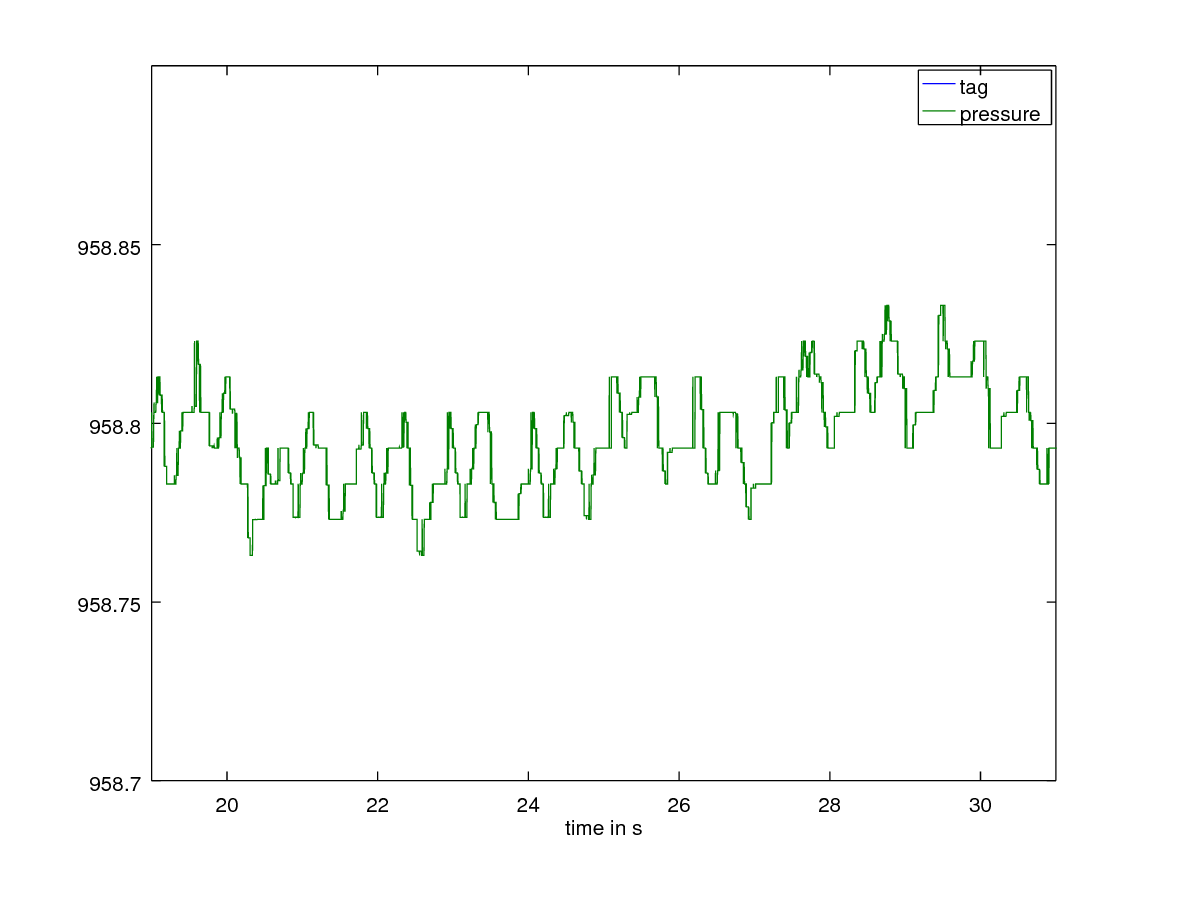
\includegraphics[width=.45\textwidth]{stairsfhdown20_walking_p} &
		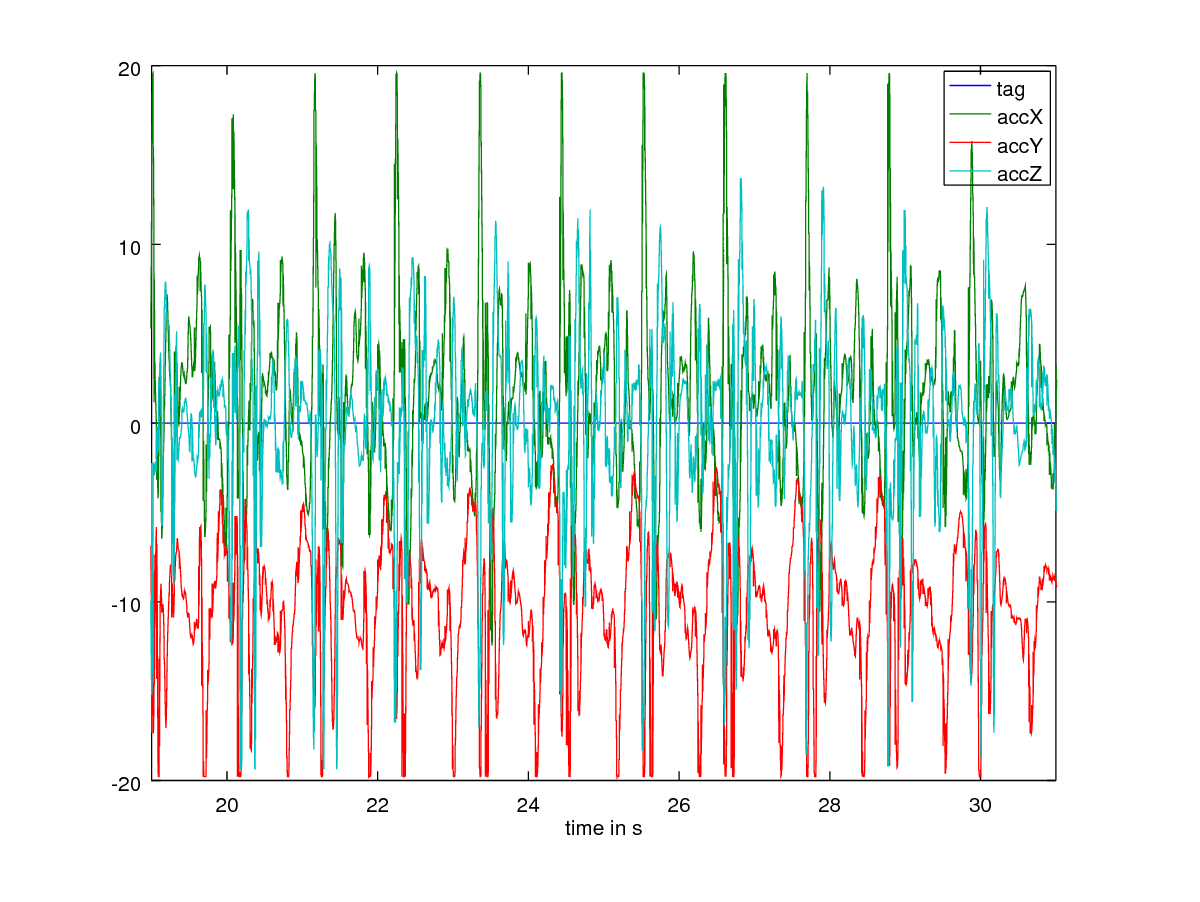
\includegraphics[width=.45\textwidth]{stairsfhdown20_walking_a} 
		\\
		(a) & (b)
		\\[4pt]	%vertical extra spacing (4 points)
		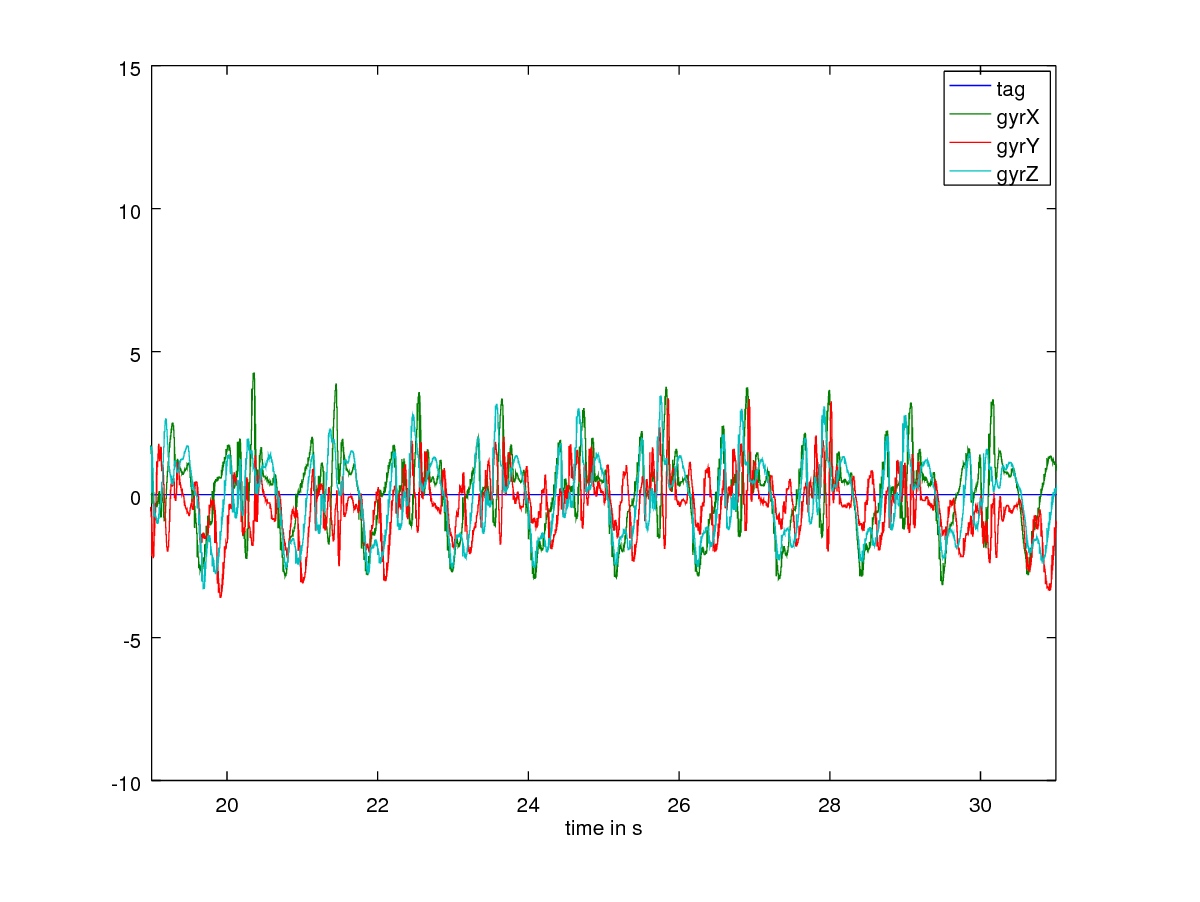
\includegraphics[width=.45\textwidth]{stairsfhdown20_walking_g} &
		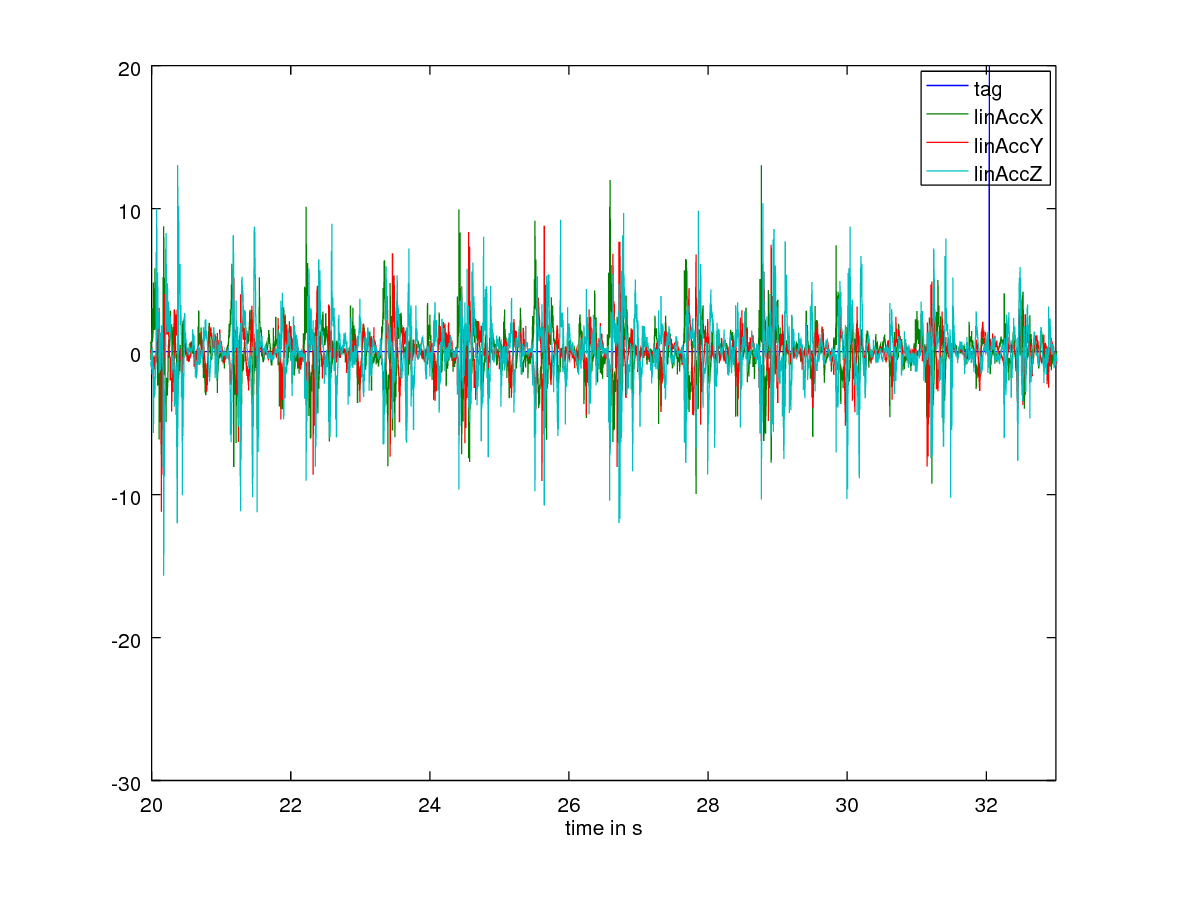
\includegraphics[width=.45\textwidth]{stairsfhdown20_walking_la} 
		\\
		(c) & (d)
		\\[4pt]	%vertical extra spacing (4 points)
		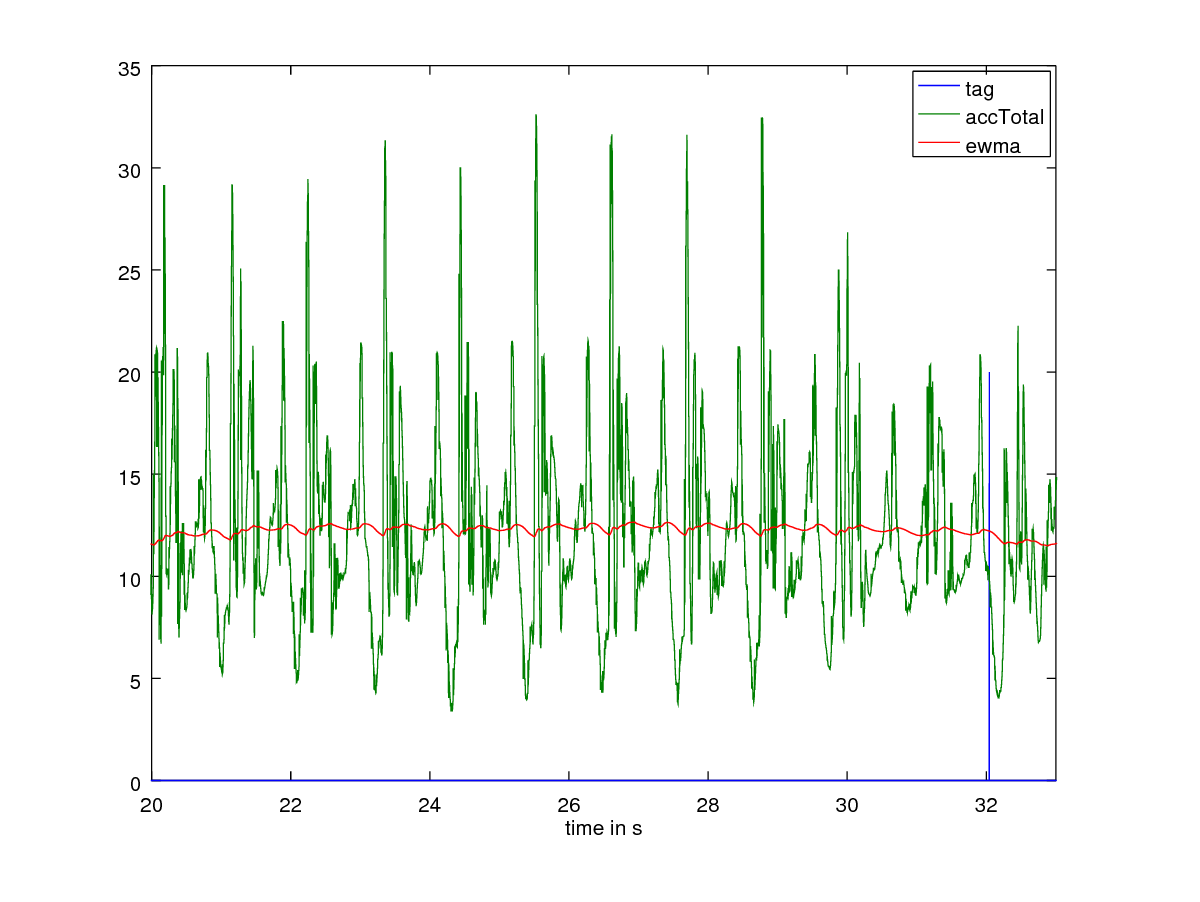
\includegraphics[width=.45\textwidth]{stairsfhdown20_walking_atotal} &
		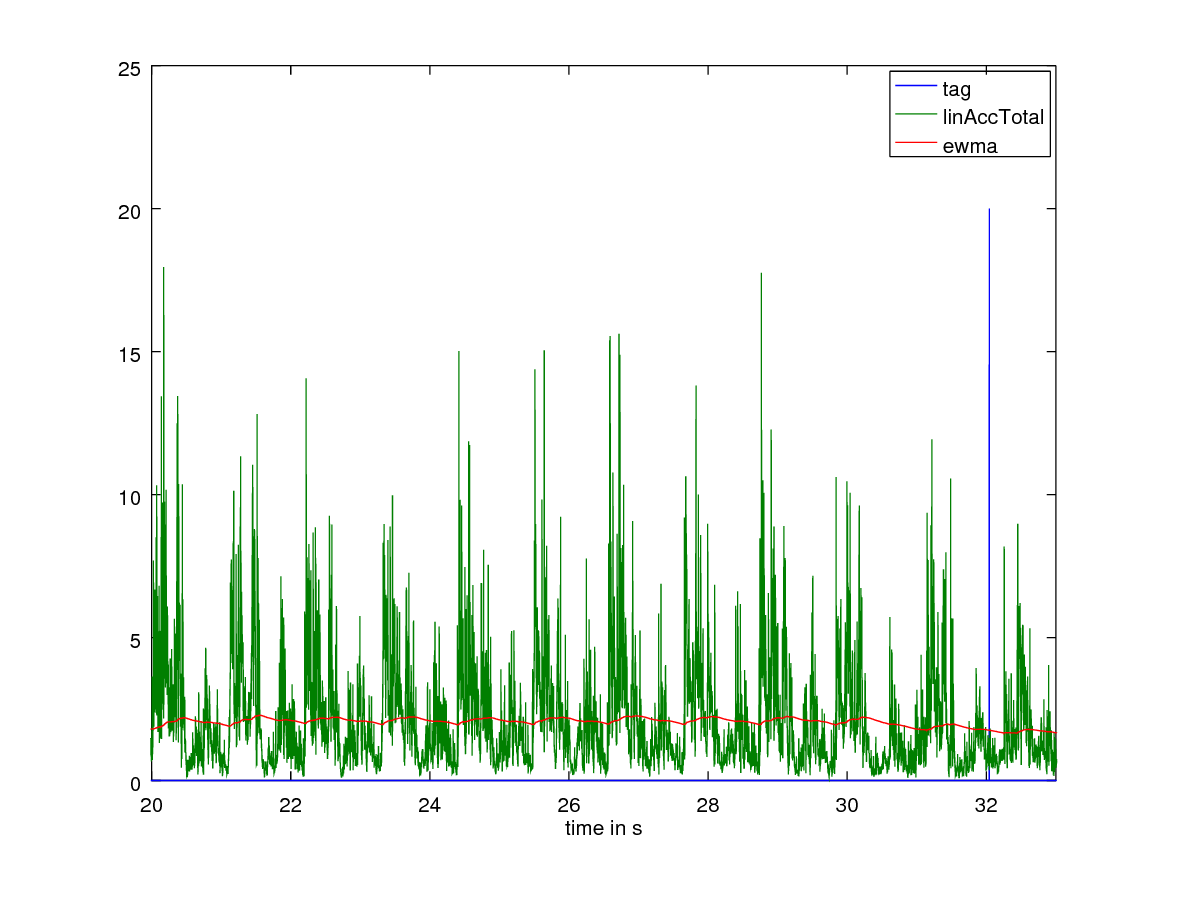
\includegraphics[width=.45\textwidth]{stairsfhdown20_walking_latotal} 
		\\
		(e) & (f)
		\end{tabular}
		%
		\caption{Test case 5}
		\label{fig:Test_case_5_walking}
	\end{figure}
	
%%%----------------------------------------------------------
\section{Test case 6}
%%%----------------------------------------------------------
Test case 6 in Fig.~\ref{fig:Test_case_6_walking}
\begin{figure}
	\centering\small
	\setlength{\tabcolsep}{0mm}	% alle Spaltenränder auf 0mm
	\begin{tabular}{c@{\hspace{12mm}}c} % mittlerer Abstand = 12mm
		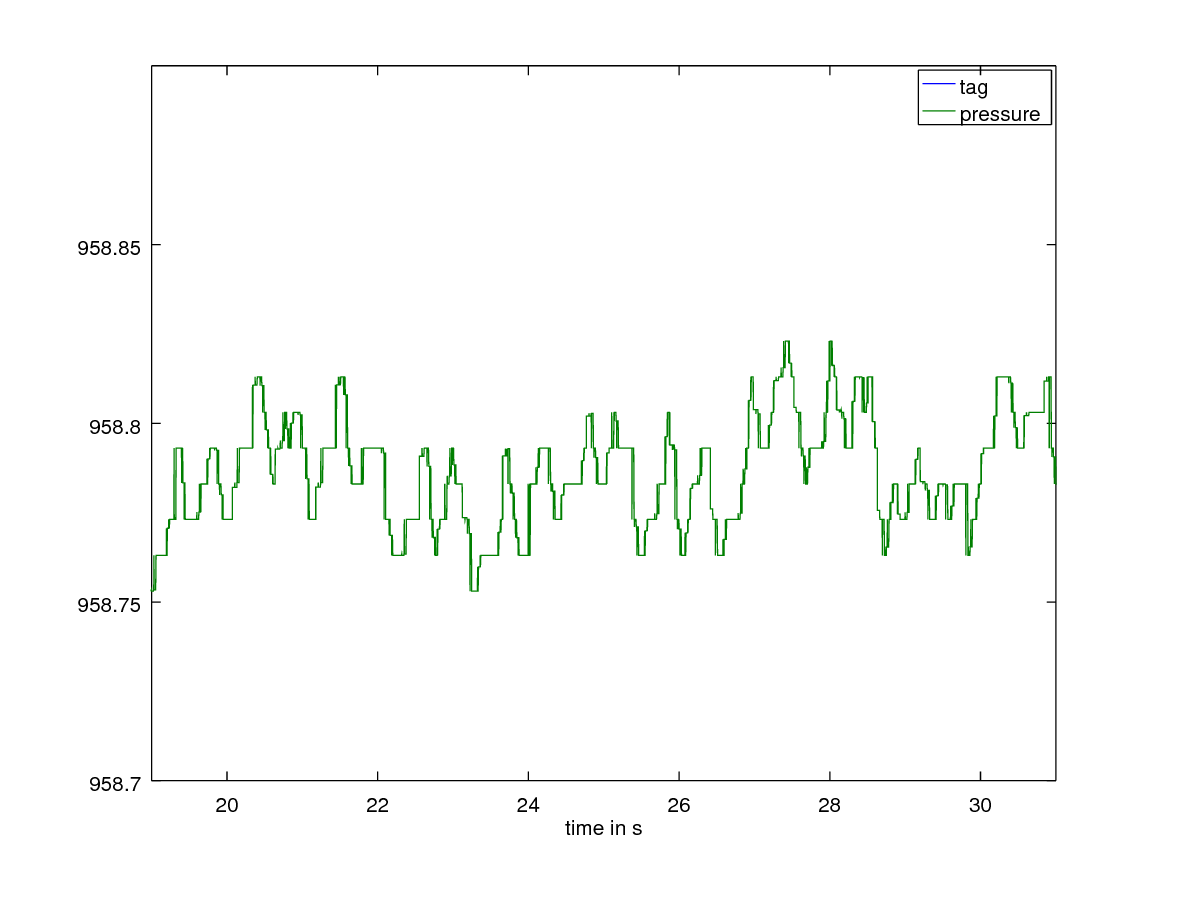
\includegraphics[width=.45\textwidth]{stairsfhdown50_walking_p} &
		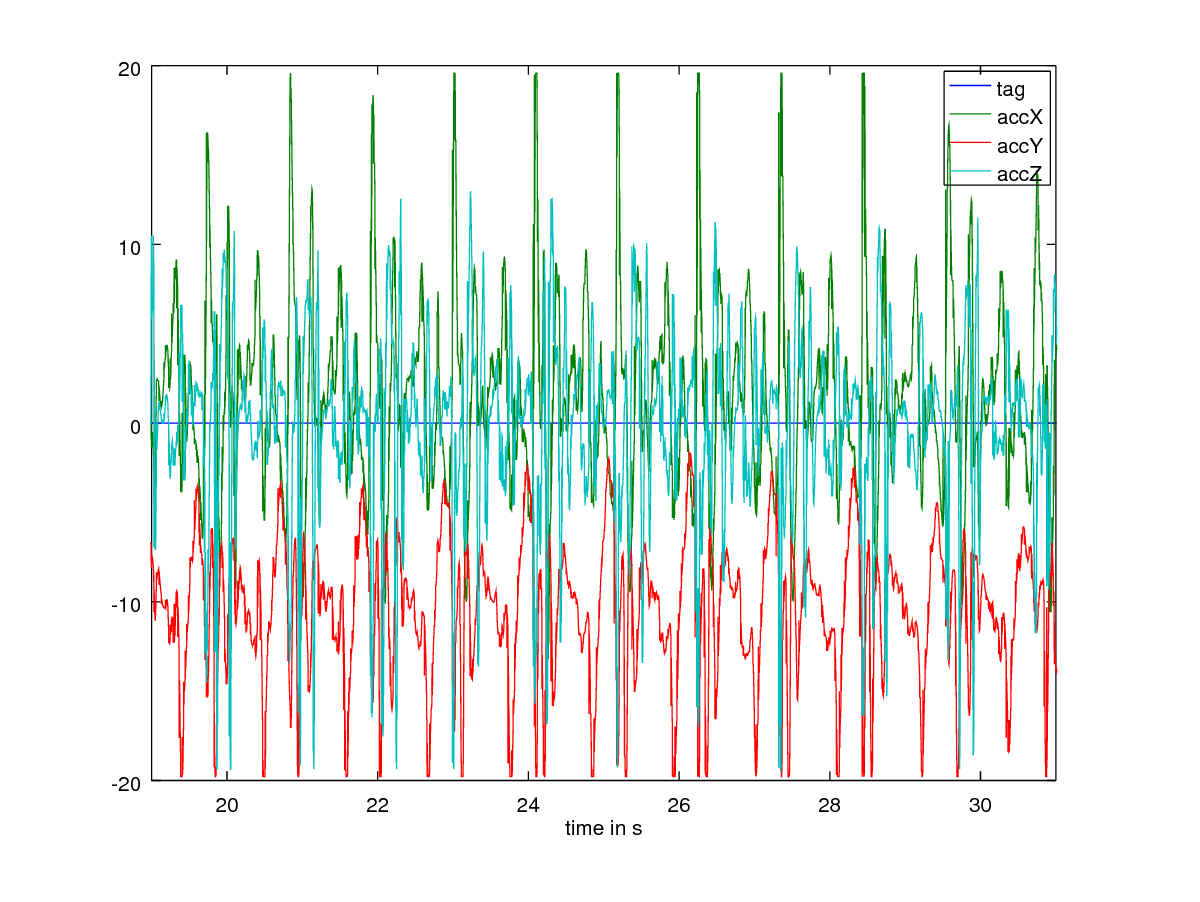
\includegraphics[width=.45\textwidth]{stairsfhdown50_walking_a} 
		\\
		(a) & (b)
		\\[4pt]	%vertical extra spacing (4 points)
		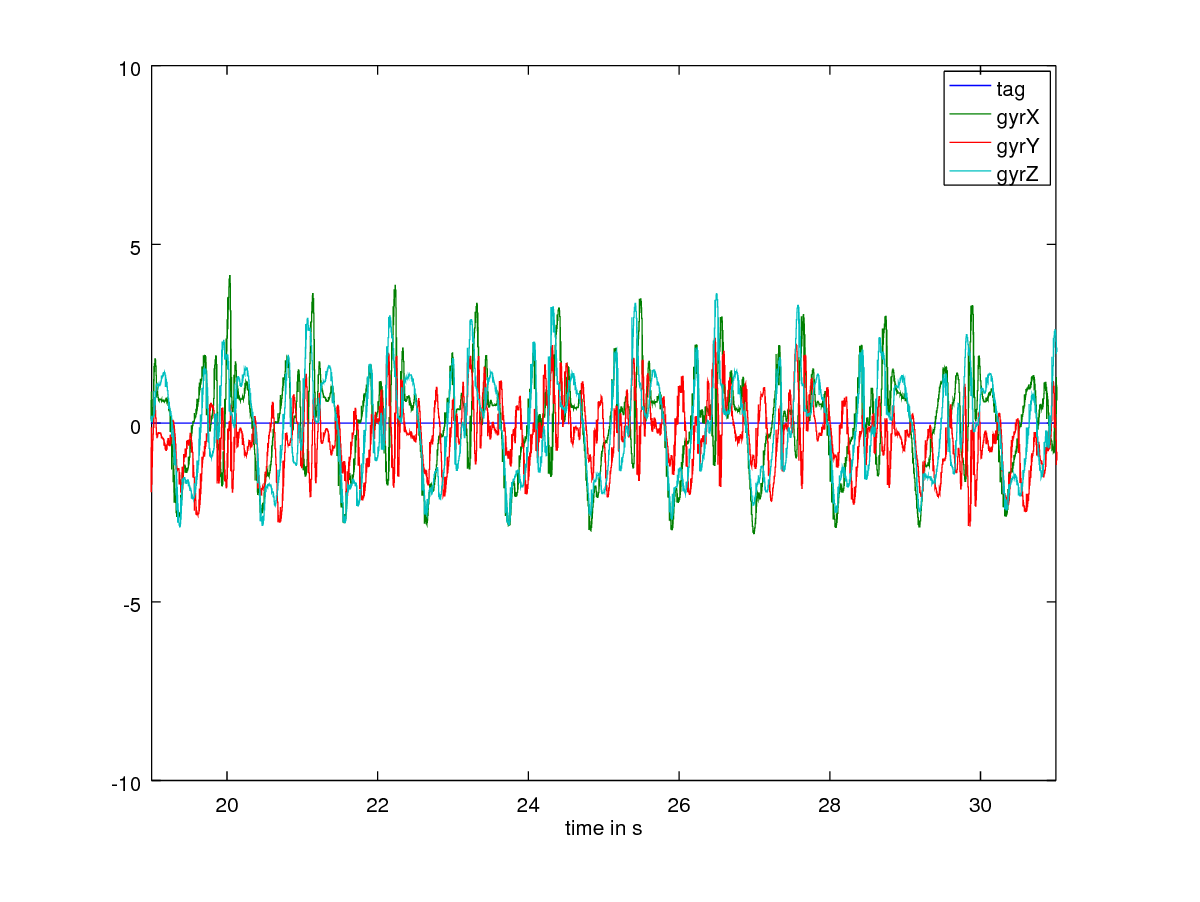
\includegraphics[width=.45\textwidth]{stairsfhdown50_walking_g} &
		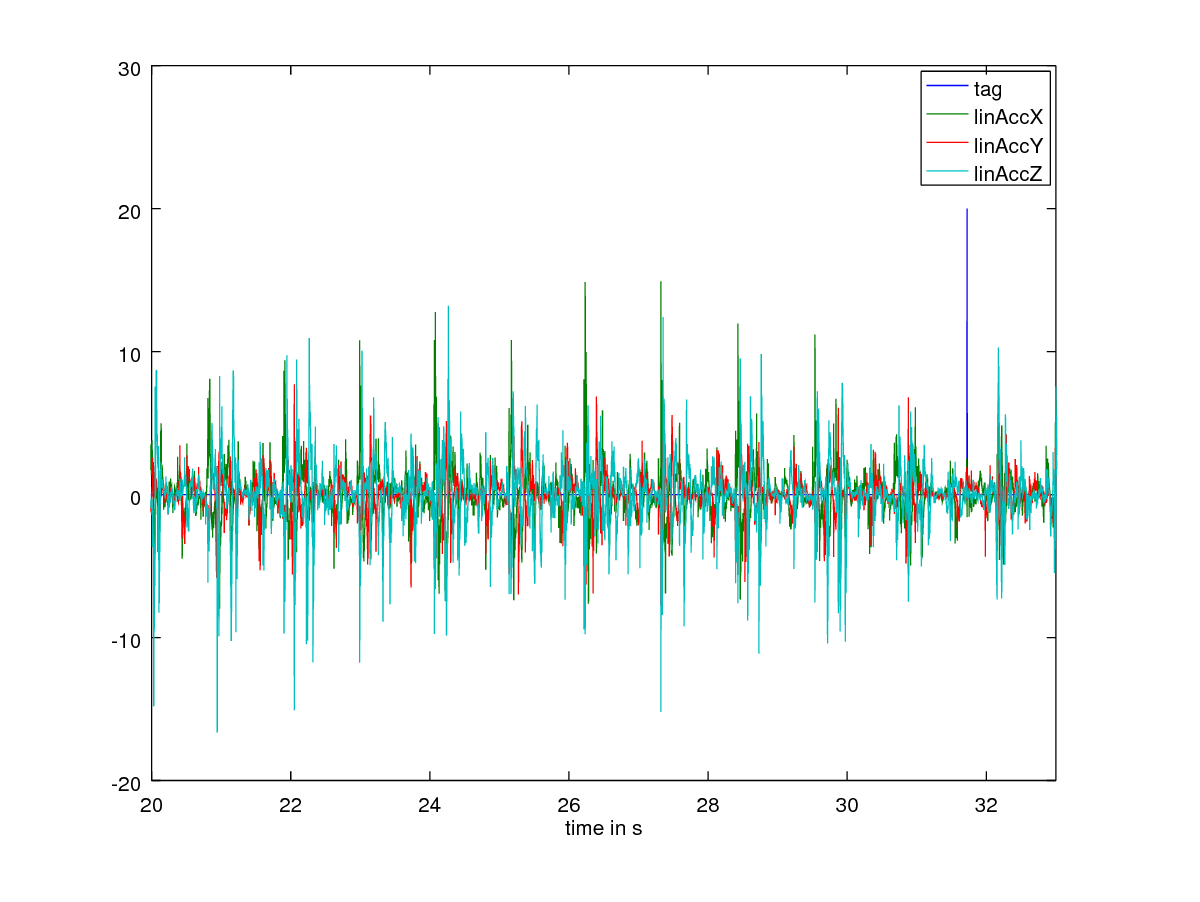
\includegraphics[width=.45\textwidth]{stairsfhdown50_walking_la} 
		\\
		(c) & (d)
		\\[4pt]	%vertical extra spacing (4 points)
		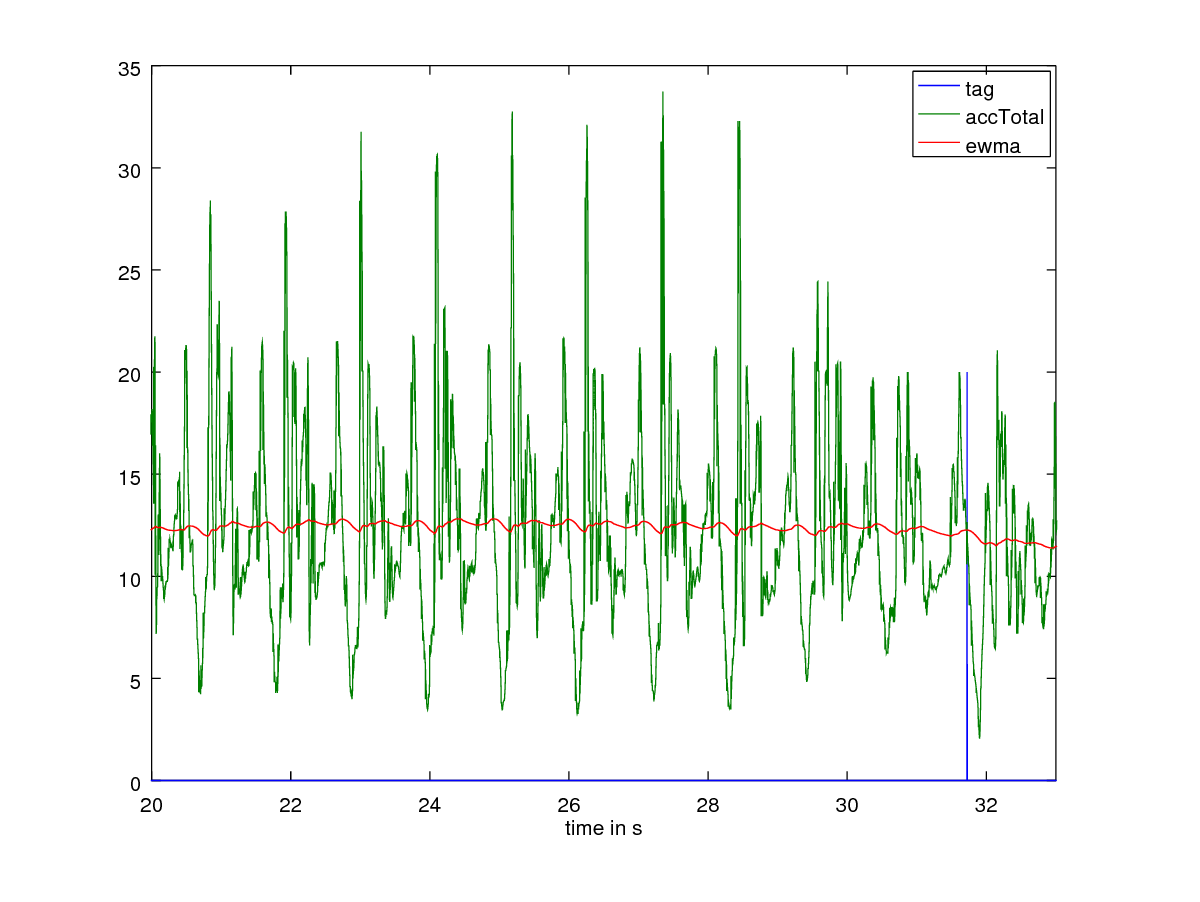
\includegraphics[width=.45\textwidth]{stairsfhdown50_walking_atotal} &
		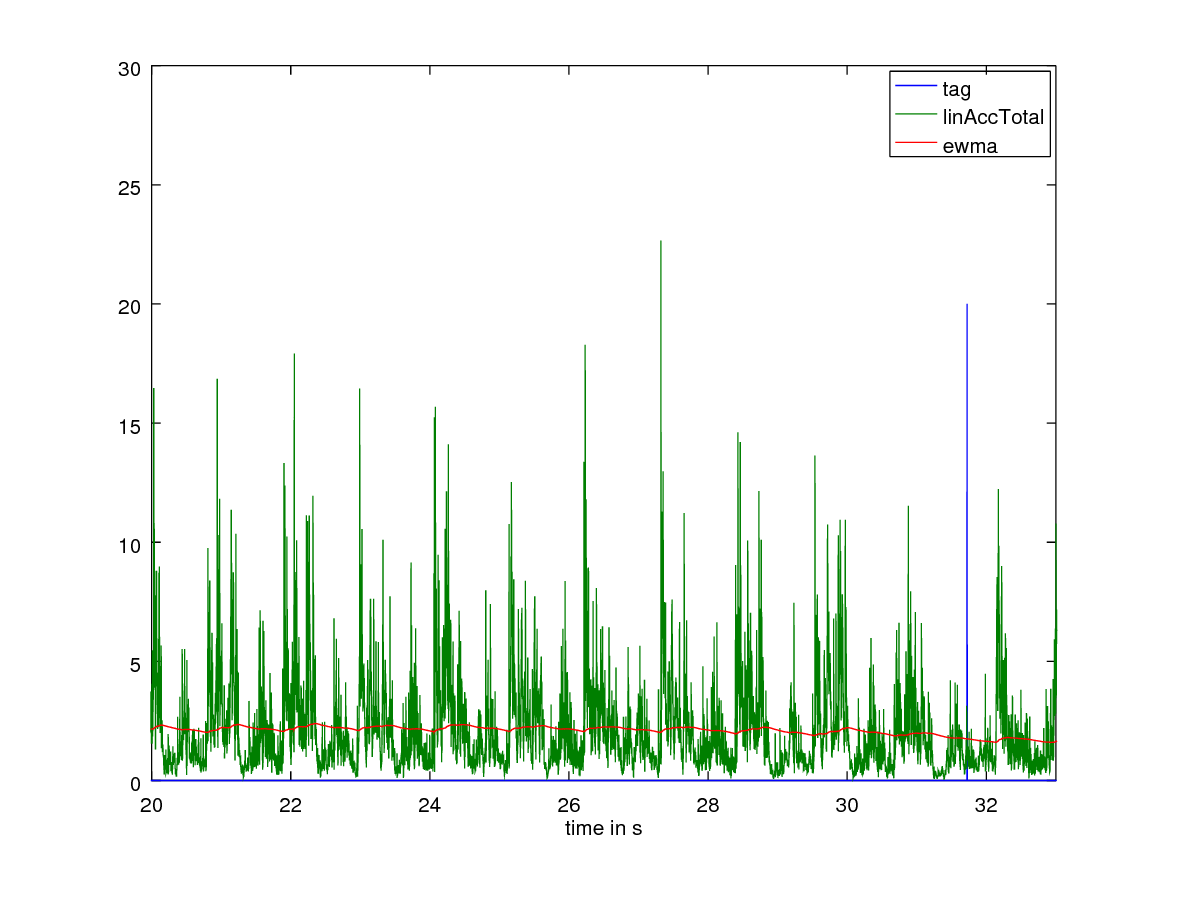
\includegraphics[width=.45\textwidth]{stairsfhdown50_walking_latotal} 
		\\
		(e) & (f)
		\end{tabular}
		%
		\caption{Test case 6}
		\label{fig:Test_case_6_walking}
	\end{figure}
	
	
%%%----------------------------------------------------------
\section{Test case 7}
%%%----------------------------------------------------------
Test case 7 in Fig.~\ref{fig:Test_case_7_walking}
\begin{figure}
	\centering\small
	\setlength{\tabcolsep}{0mm}	% alle Spaltenränder auf 0mm
	\begin{tabular}{c@{\hspace{12mm}}c} % mittlerer Abstand = 12mm
		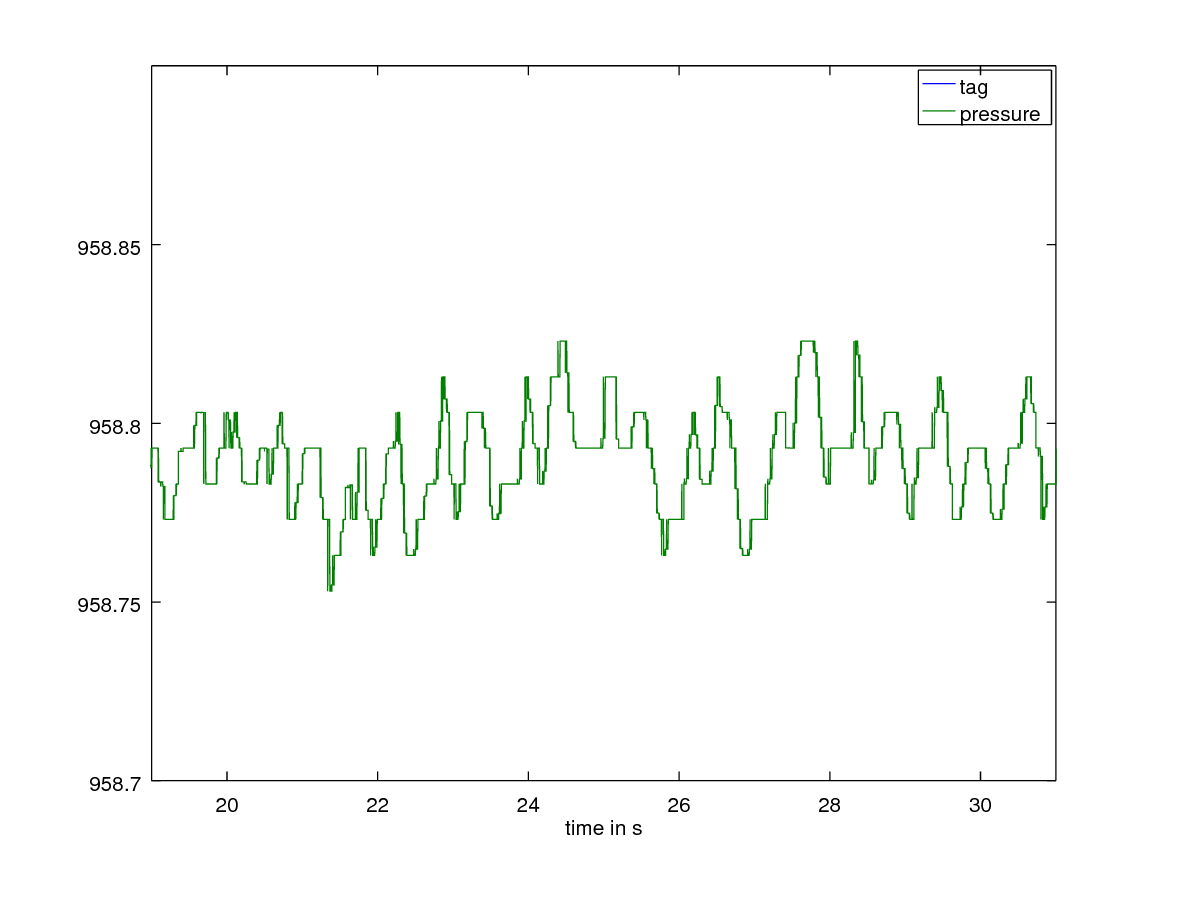
\includegraphics[width=.45\textwidth]{stairsfhdown70_walking_p} &
		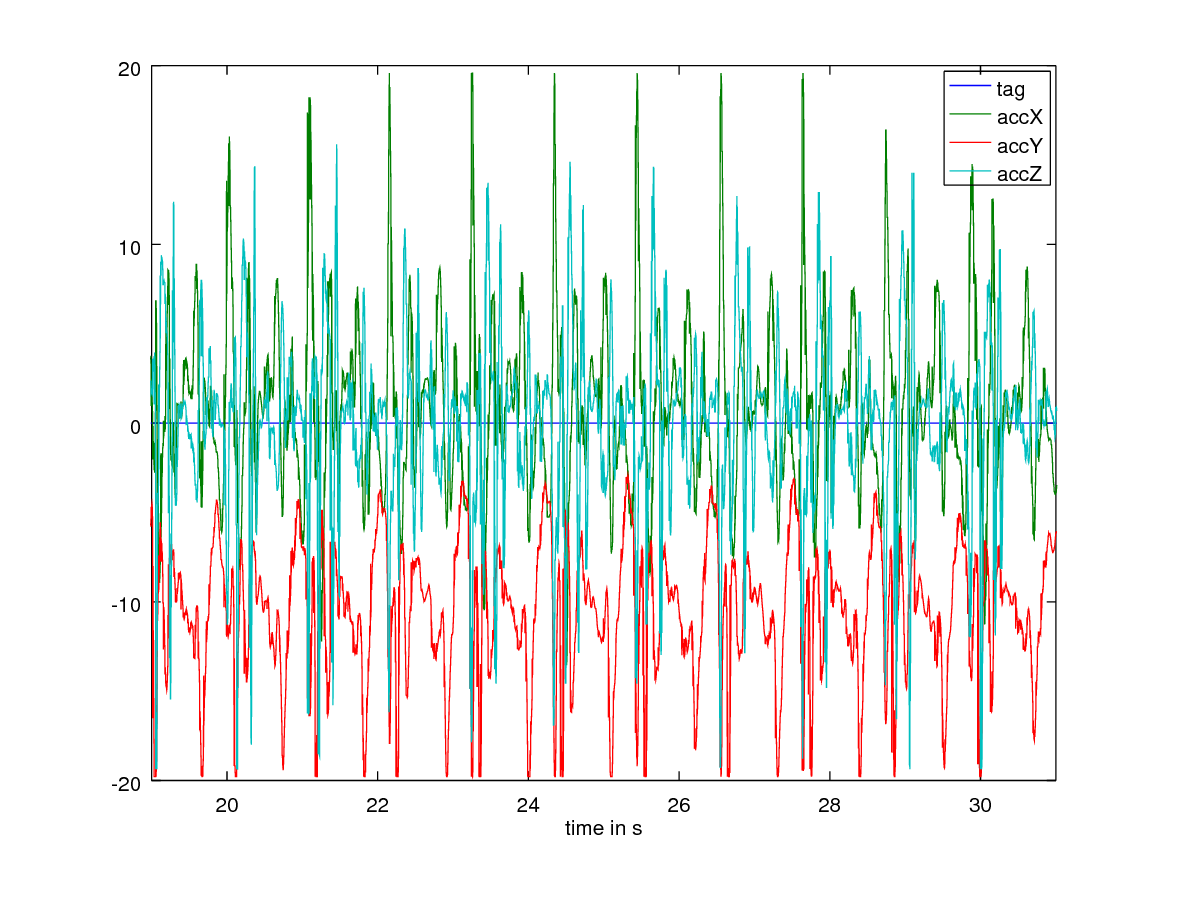
\includegraphics[width=.45\textwidth]{stairsfhdown70_walking_a} 
		\\
		(a) & (b)
		\\[4pt]	%vertical extra spacing (4 points)
		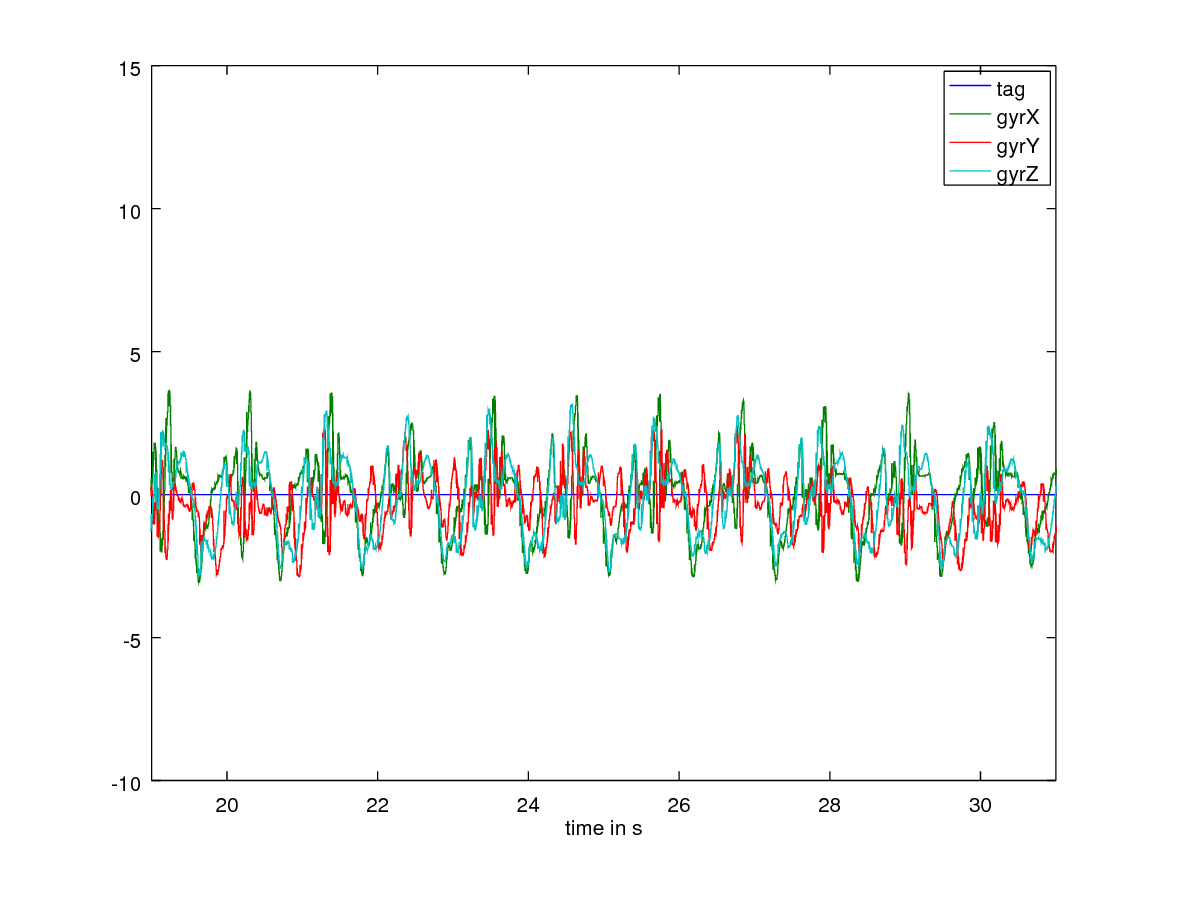
\includegraphics[width=.45\textwidth]{stairsfhdown70_walking_g} &
		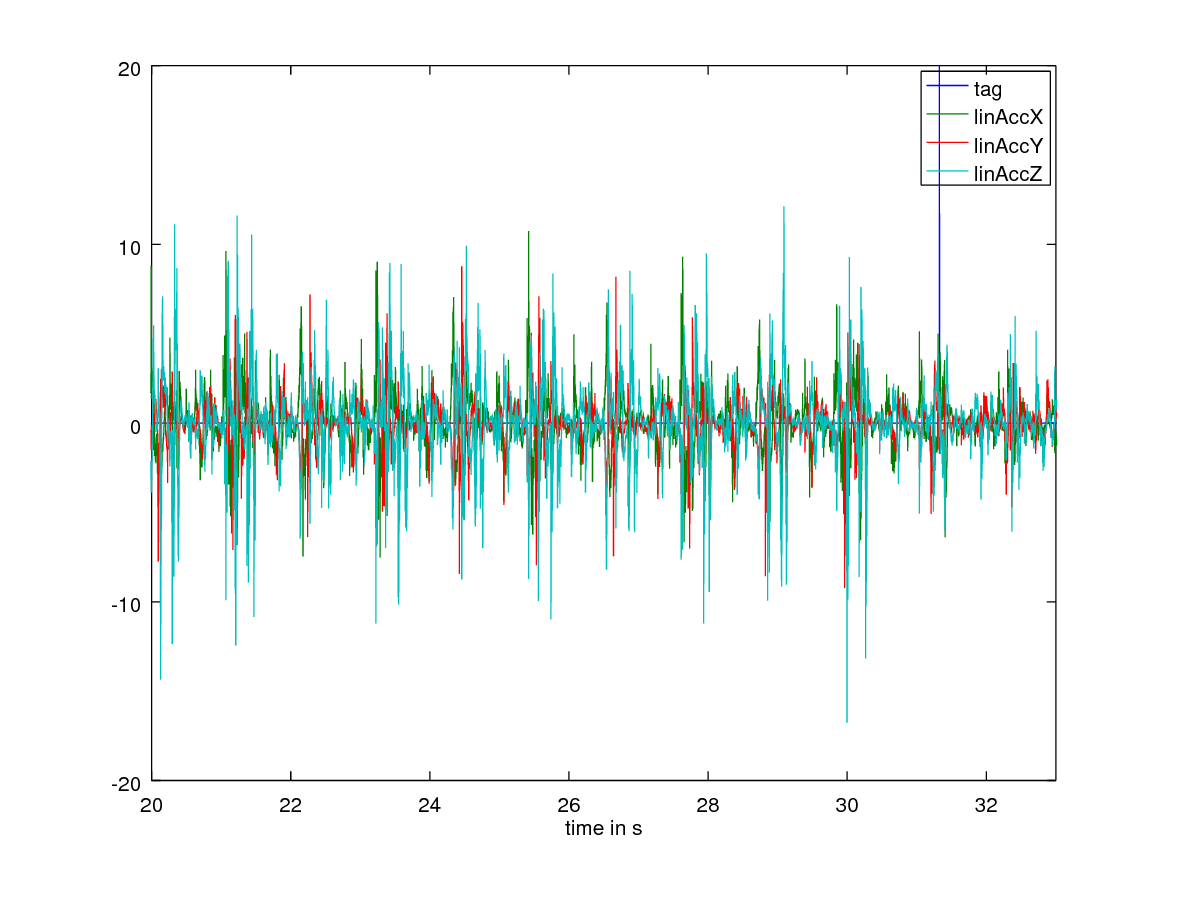
\includegraphics[width=.45\textwidth]{stairsfhdown70_walking_la} 
		\\
		(c) & (d)
		\\[4pt]	%vertical extra spacing (4 points)
		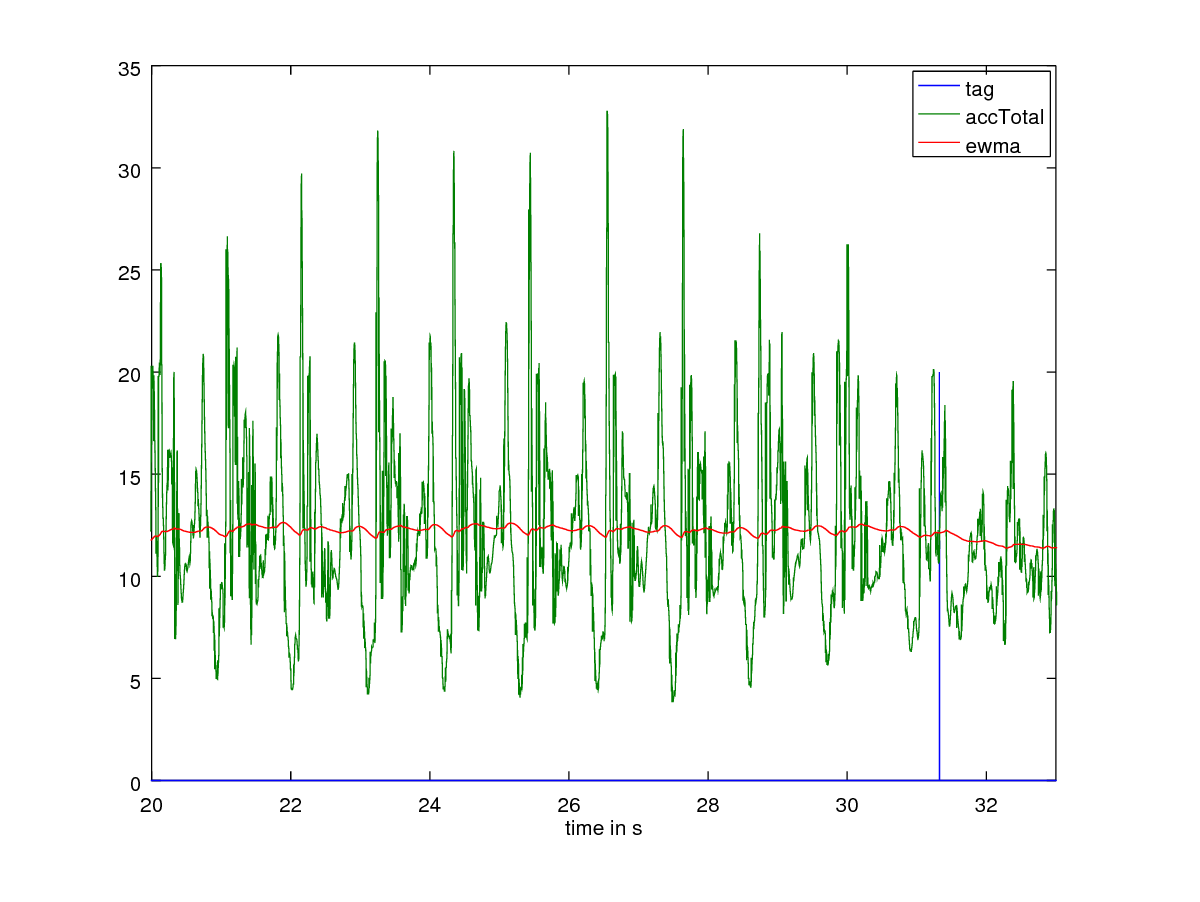
\includegraphics[width=.45\textwidth]{stairsfhdown70_walking_atotal} &
		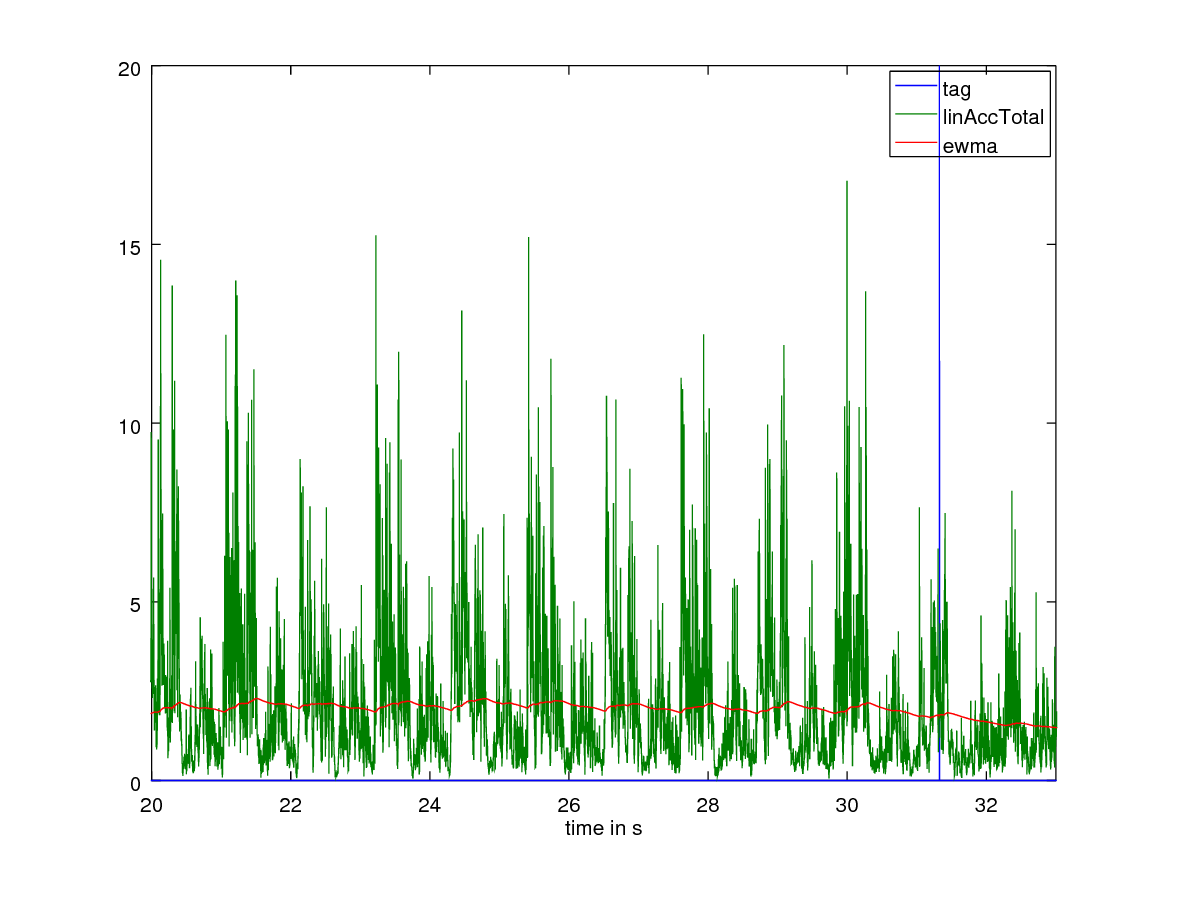
\includegraphics[width=.45\textwidth]{stairsfhdown70_walking_latotal} 
		\\
		(e) & (f)
		\end{tabular}
		%
		\caption{Test case 7}
		\label{fig:Test_case_7_walking}
	\end{figure}
	
	
%%%----------------------------------------------------------
\section{Test case 8}
%%%----------------------------------------------------------
Test case 8 in Fig.~\ref{fig:Test_case_8_walking}
\begin{figure}
	\centering\small
	\setlength{\tabcolsep}{0mm}	% alle Spaltenränder auf 0mm
	\begin{tabular}{c@{\hspace{12mm}}c} % mittlerer Abstand = 12mm
		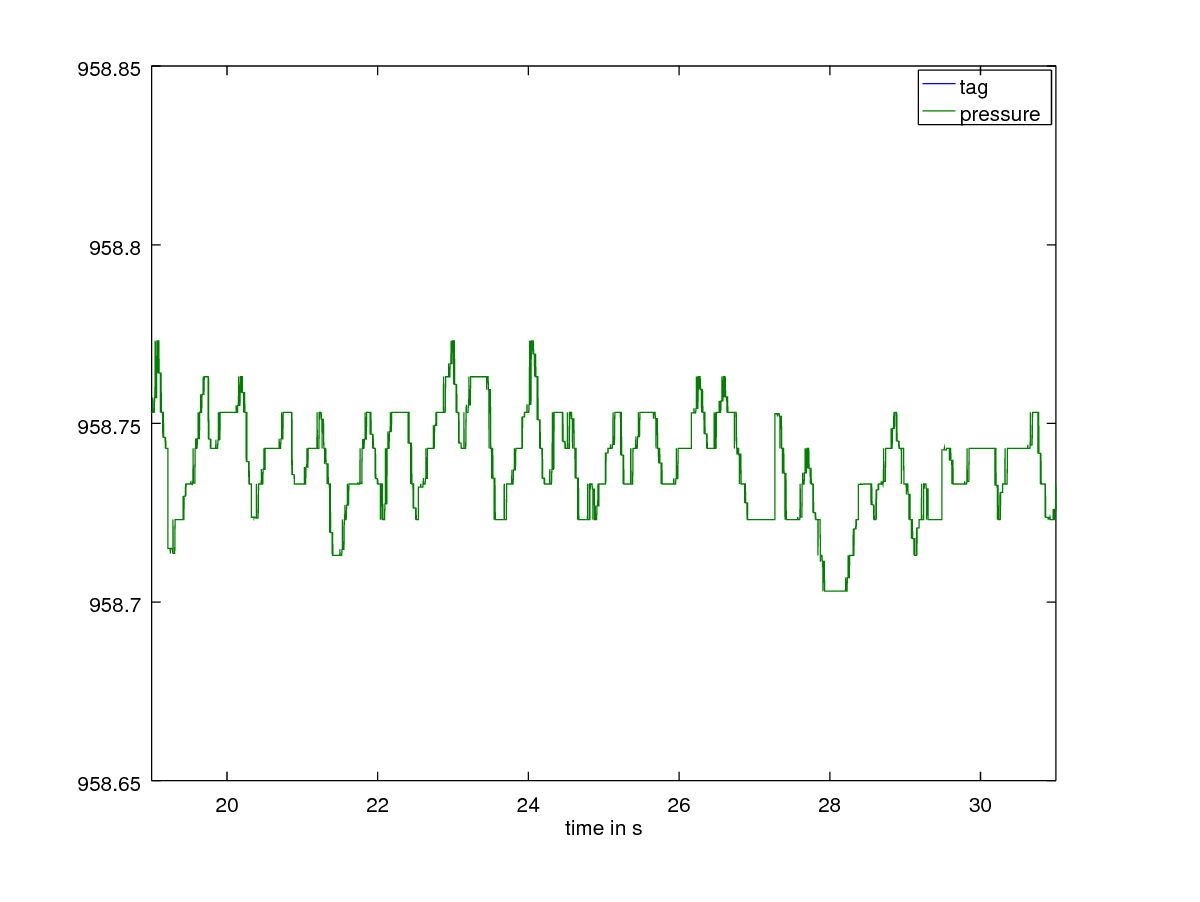
\includegraphics[width=.45\textwidth]{stairsfhdown100_walking_p} &
		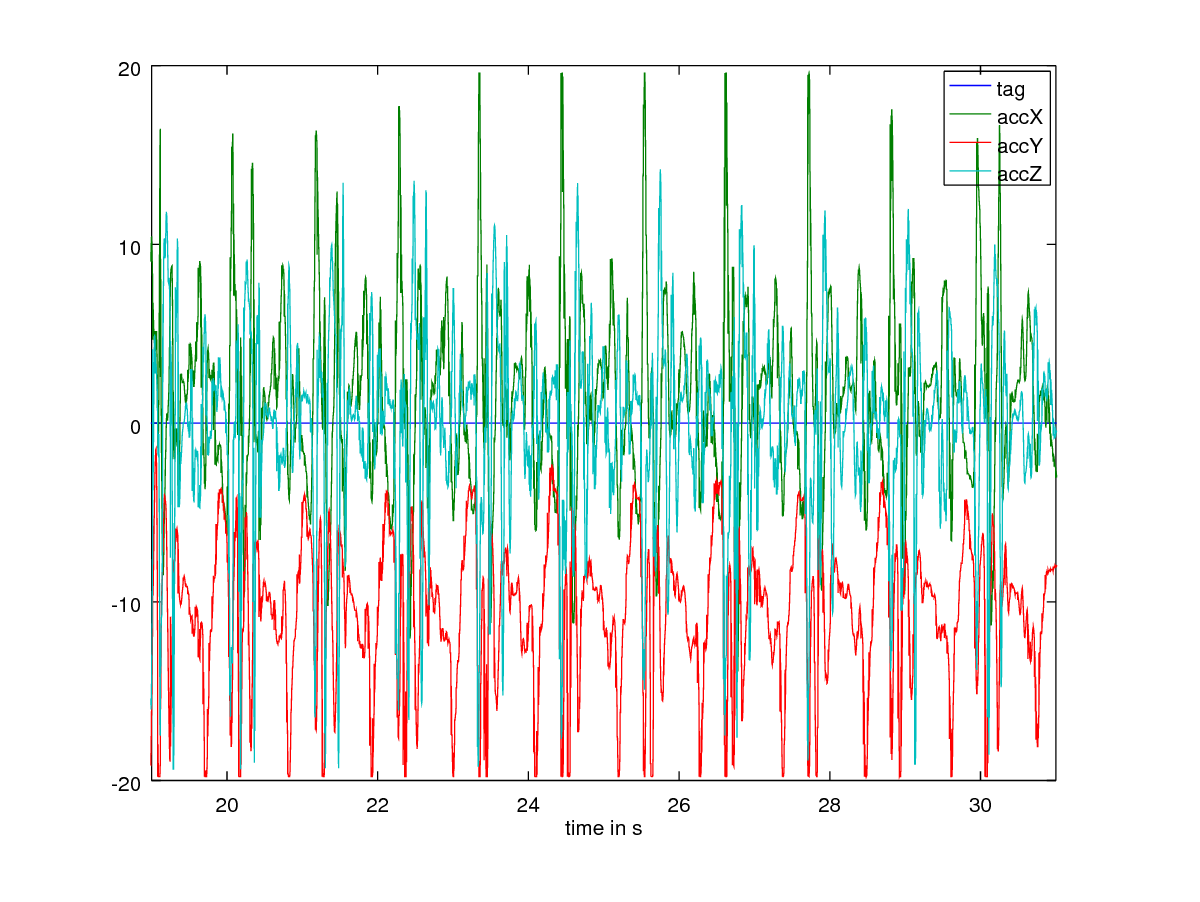
\includegraphics[width=.45\textwidth]{stairsfhdown100_walking_a} 
		\\
		(a) & (b)
		\\[4pt]	%vertical extra spacing (4 points)
		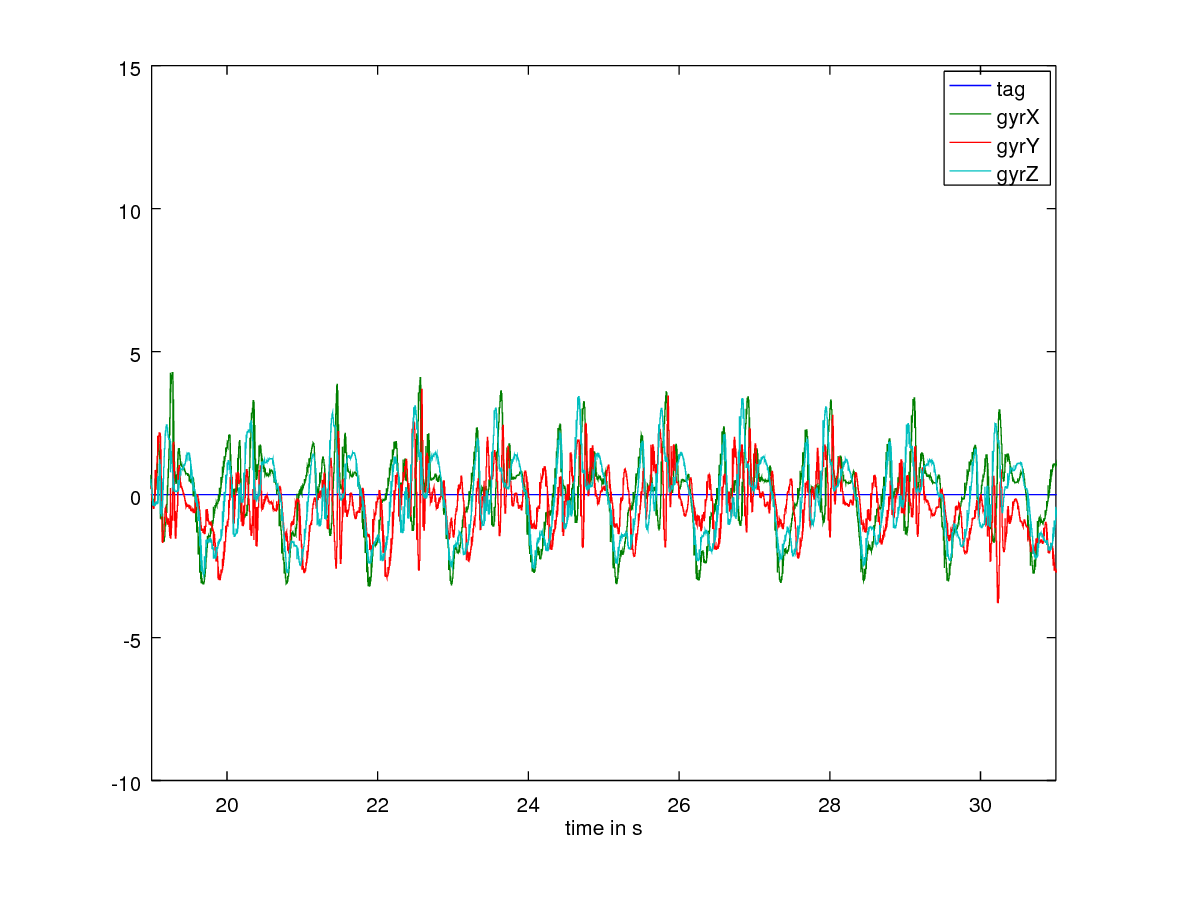
\includegraphics[width=.45\textwidth]{stairsfhdown100_walking_g} &
		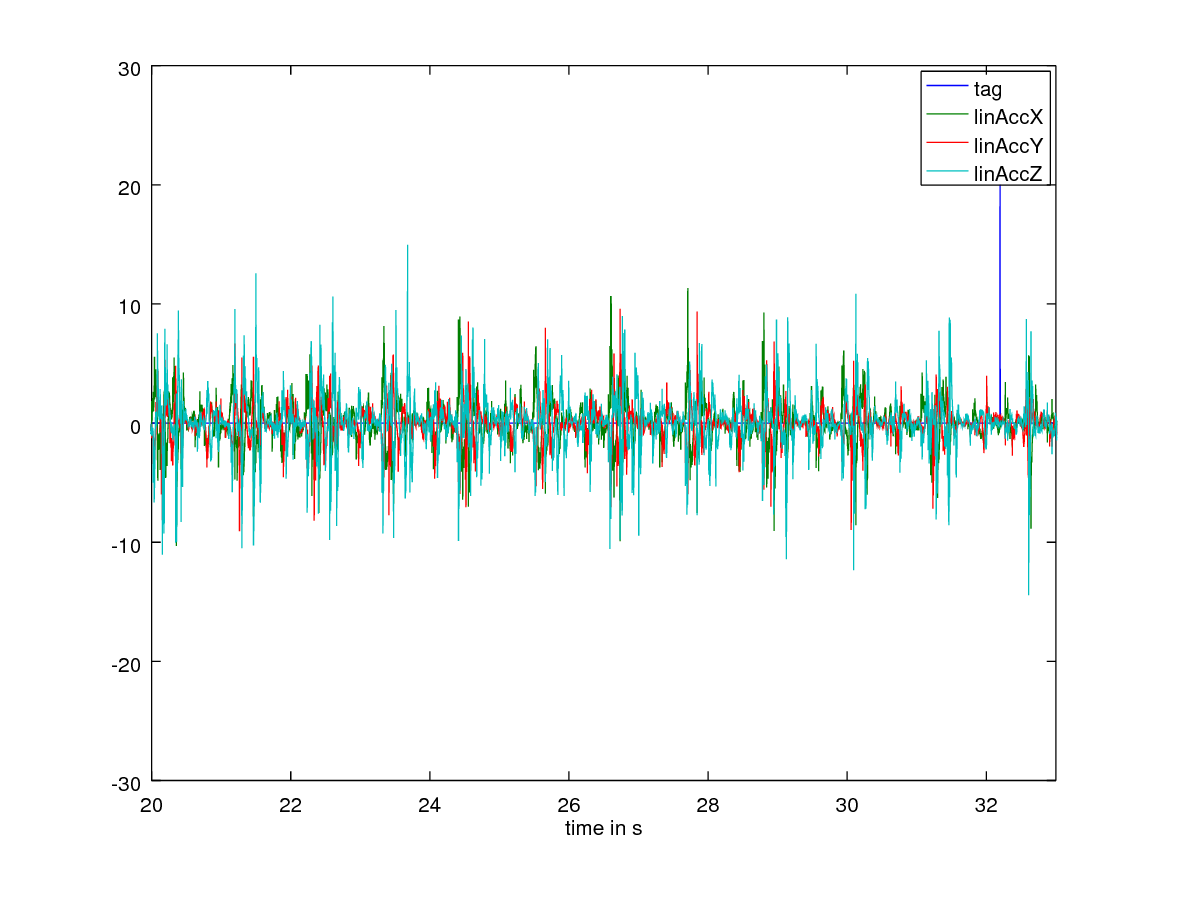
\includegraphics[width=.45\textwidth]{stairsfhdown100_walking_la} 
		\\
		(c) & (d)
		\\[4pt]	%vertical extra spacing (4 points)
		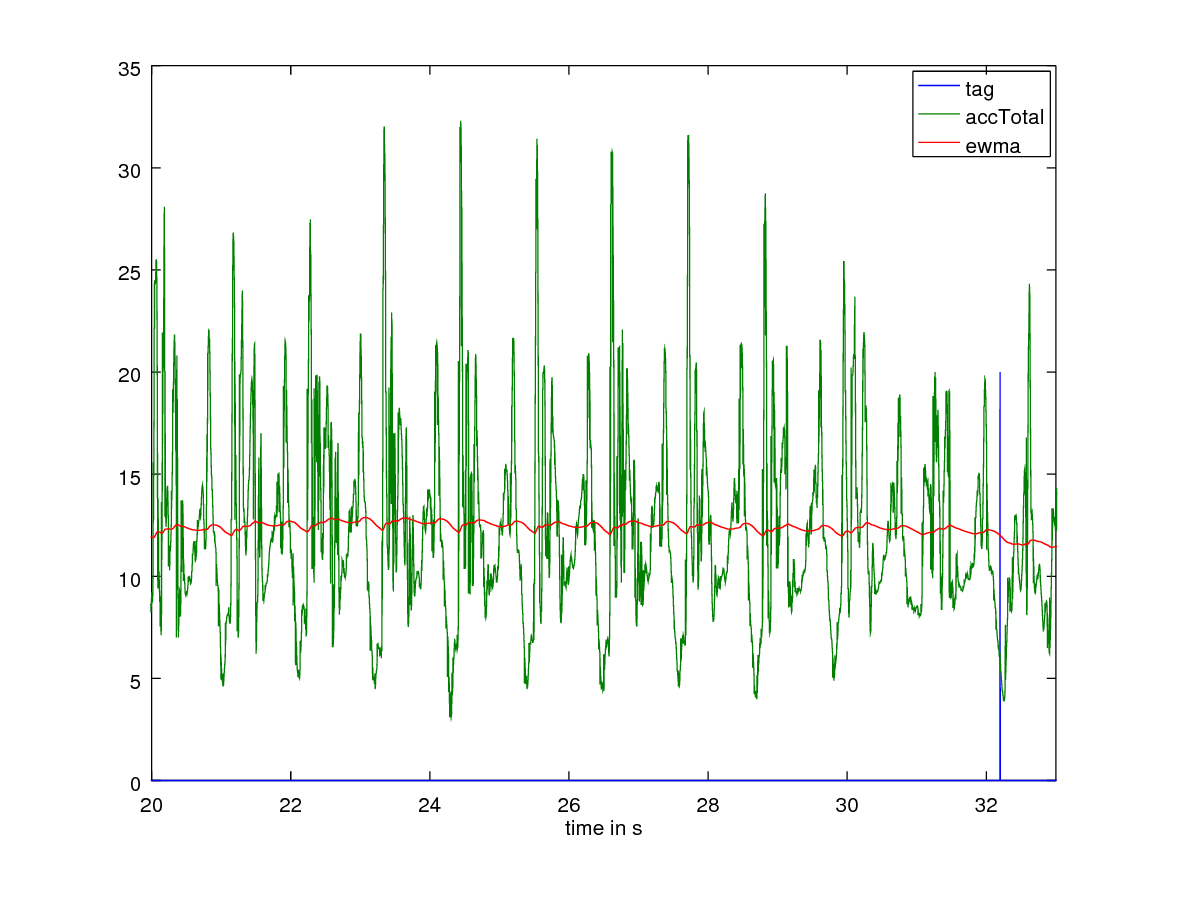
\includegraphics[width=.45\textwidth]{stairsfhdown100_walking_atotal} &
		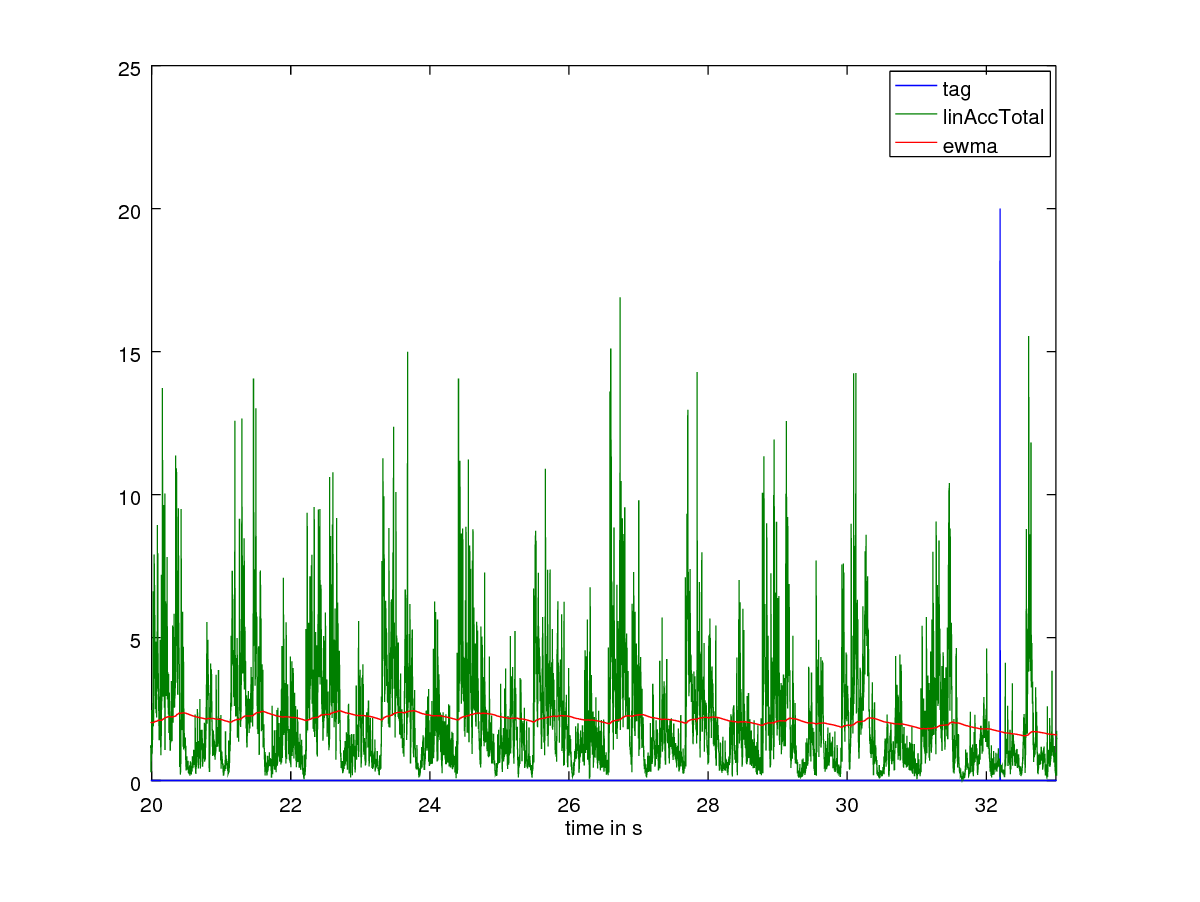
\includegraphics[width=.45\textwidth]{stairsfhdown100_walking_latotal} 
		\\
		(e) & (f)
		\end{tabular}
		%
		\caption{Test case 8}
		\label{fig:Test_case_8_walking}
	\end{figure}
	
%%%----------------------------------------------------------
\section{Test case 9}
%%%----------------------------------------------------------
Test case 9 in Fig.~\ref{fig:Test_case_9_walking}
\begin{figure}
	\centering\small
	\setlength{\tabcolsep}{0mm}	% alle Spaltenränder auf 0mm
	\begin{tabular}{c@{\hspace{12mm}}c} % mittlerer Abstand = 12mm
		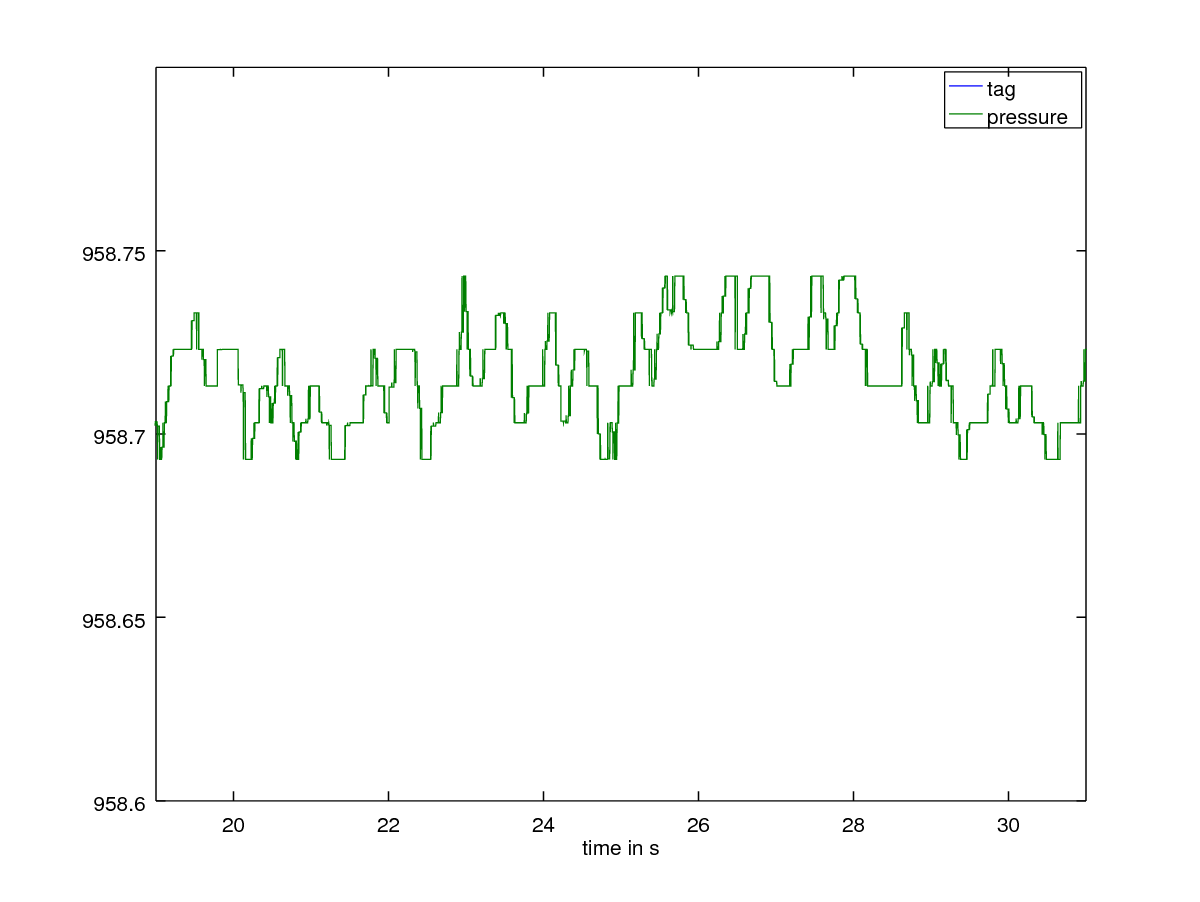
\includegraphics[width=.45\textwidth]{stairsfhdowna2_walking_p} &
		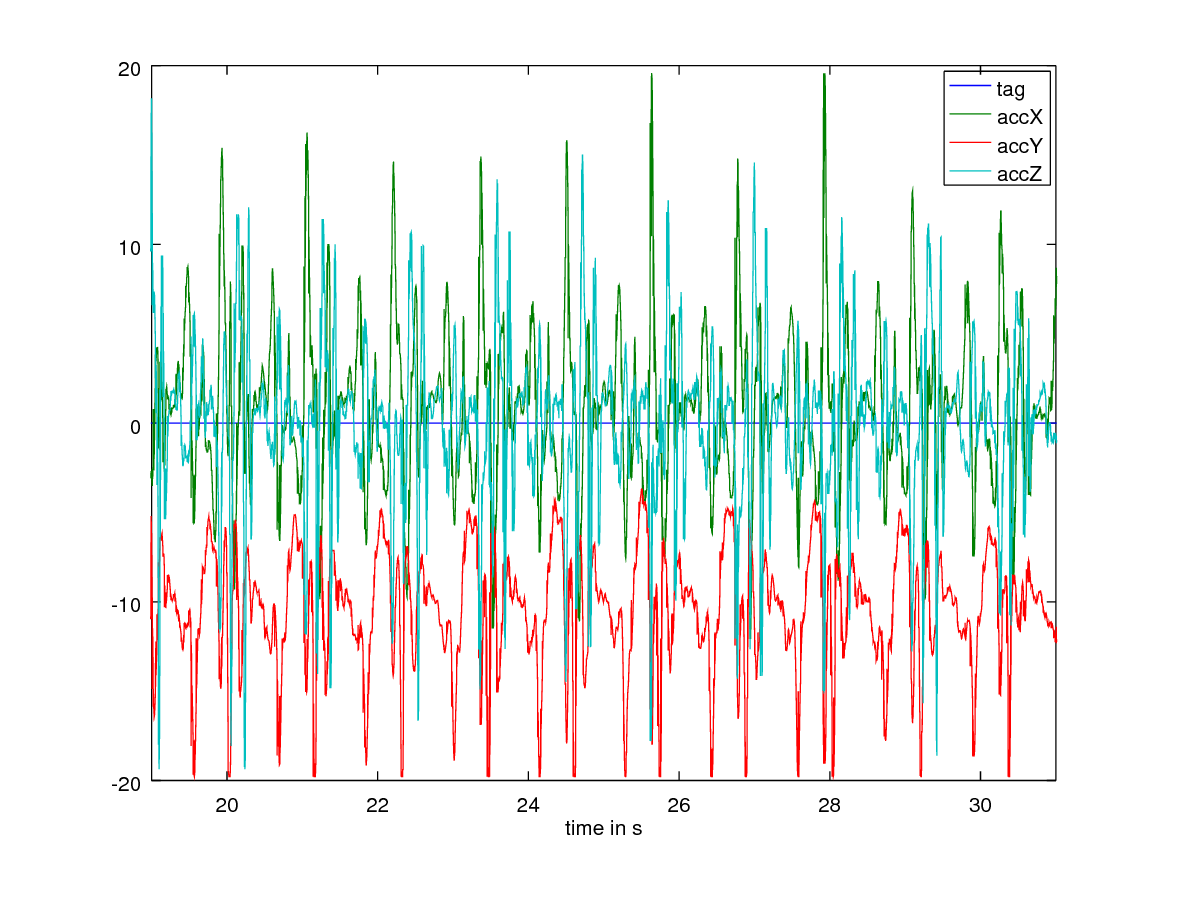
\includegraphics[width=.45\textwidth]{stairsfhdowna2_walking_a} 
		\\
		(a) & (b)
		\\[4pt]	%vertical extra spacing (4 points)
		\includegraphics[width=.45\textwidth]{stairsfhdowna2_walking_g} &
		\includegraphics[width=.45\textwidth]{stairsfhdowna2_walking_la} 
		\\
		(c) & (d)
		\\[4pt]	%vertical extra spacing (4 points)
		\includegraphics[width=.45\textwidth]{stairsfhdowna2_walking_atotal} &
		\includegraphics[width=.45\textwidth]{stairsfhdowna2_walking_latotal} 
		\\
		(e) & (f)
		\end{tabular}
		%
		\caption{Test case 9}
		\label{fig:Test_case_9_walking}
	\end{figure}
	
%%%----------------------------------------------------------
\section{Test case 10}
%%%----------------------------------------------------------
Test case 10 in Fig.~\ref{fig:Test_case_10_walking}
\begin{figure}
	\centering\small
	\setlength{\tabcolsep}{0mm}	% alle Spaltenränder auf 0mm
	\begin{tabular}{c@{\hspace{12mm}}c} % mittlerer Abstand = 12mm
		\includegraphics[width=.45\textwidth]{stairsfhdownf1_walking_p} &
		\includegraphics[width=.45\textwidth]{stairsfhdownf1_walking_a} 
		\\
		(a) & (b)
		\\[4pt]	%vertical extra spacing (4 points)
		\includegraphics[width=.45\textwidth]{stairsfhdownf1_walking_g} &
		\includegraphics[width=.45\textwidth]{stairsfhdownf1_walking_la} 
		\\
		(c) & (d)
		\\[4pt]	%vertical extra spacing (4 points)
		\includegraphics[width=.45\textwidth]{stairsfhdownf1_walking_atotal} &
		\includegraphics[width=.45\textwidth]{stairsfhdownf1_walking_latotal} 
		\\
		(e) & (f)
		\end{tabular}
		%
		\caption{Test case 10}
		\label{fig:Test_case_10_walking}
	\end{figure}